%==============================================================================
% tento soubor pouzijte jako zaklad
% this file should be used as a base for the thesis
% Autoři / Authors: 2008 Michal Bidlo, 2016 Jaroslav Dytrych
% Kontakt pro dotazy a připomínky: dytrych@fit.vutbr.cz
% Contact for questions and comments: dytrych@fit.vutbr.cz
%==============================================================================
% kodovani: UTF-8 (zmena prikazem iconv, recode nebo cstocs)
% encoding: UTF-8 (you can change it by command iconv, recode or cstocs)
%------------------------------------------------------------------------------
% zpracování / processing: make, make pdf, make clean
%==============================================================================
% Soubory, které je nutné upravit: / Files which have to be edited:
%   projekt-20-literatura-bibliography.bib - literatura / bibliography
%   projekt-01-kapitoly-chapters.tex - obsah práce / the thesis content
%   projekt-30-prilohy-appendices.tex - přílohy / appendices
%==============================================================================
%\documentclass[]{fitthesis} % bez zadání - pro začátek práce, aby nebyl problém s překladem
%\documentclass[english]{fitthesis} % without assignment - for the work start to avoid compilation problem
\documentclass[slovak]{fitthesis} % odevzdani do wisu - odkazy jsou barevné
%\documentclass[english,zadani]{fitthesis} % for submission to the IS FIT - links are color
%\documentclass[zadani,print]{fitthesis} % pro tisk - odkazy jsou černé
%\documentclass[zadani,cprint]{fitthesis} % pro barevný tisk - odkazy jsou černé, znak VUT barevný
%\documentclass[english,zadani,print]{fitthesis} % for the color print - links are black
%\documentclass[english,zadani,cprint]{fitthesis} % for the print - links are black, logo is color
% * Je-li práce psaná v anglickém jazyce, je zapotřebí u třídy použít 
%   parametr english následovně:
%   If thesis is written in english, it is necessary to use 
%   parameter english as follows:
%      \documentclass[english]{fitthesis}
% * Je-li práce psaná ve slovenském jazyce, je zapotřebí u třidy použít 
%   parametr slovak následovně:
%      \documentclass[slovak]{fitthesis}

% Základní balíčky jsou dole v souboru šablony fitthesis.cls
% Basic packages are at the bottom of template file fitthesis.cls
% zde můžeme vložit vlastní balíčky / you can place own packages here

% Kompilace po částech (rychlejší, ale v náhledu nemusí být vše aktuální)
% Compilation piecewise (faster, but not all parts in preview will be up-to-date)
% \usepackage{subfiles}

% Nastavení cesty k obrázkům
% Setting of a path to the pictures
%\graphicspath{{obrazky-figures/}{./obrazky-figures/}}
%\graphicspath{{obrazky-figures/}{../obrazky-figures/}}

%---rm---------------
\renewcommand{\rmdefault}{lmr}%zavede Latin Modern Roman jako rm / set Latin Modern Roman as rm
%---sf---------------
\renewcommand{\sfdefault}{qhv}%zavede TeX Gyre Heros jako sf
%---tt------------
\renewcommand{\ttdefault}{lmtt}% zavede Latin Modern tt jako tt

% vypne funkci šablony, která automaticky nahrazuje uvozovky,
% aby nebyly prováděny nevhodné náhrady v popisech API apod.
% disables function of the template which replaces quotation marks
% to avoid unnecessary replacements in the API descriptions etc.
\csdoublequotesoff

% =======================================================================
% balíček "hyperref" vytváří klikací odkazy v pdf, pokud tedy použijeme pdflatex
% problém je, že balíček hyperref musí být uveden jako poslední, takže nemůže
% být v šabloně
% "hyperref" package create clickable links in pdf if you are using pdflatex.
% Problem is that this package have to be introduced as the last one so it 
% can not be placed in the template file.
\ifWis
\ifx\pdfoutput\undefined % nejedeme pod pdflatexem / we are not using pdflatex
\else
  \usepackage{color}
  \usepackage[unicode,colorlinks,hyperindex,plainpages=false,pdftex]{hyperref}
  \definecolor{links}{rgb}{0.4,0.5,0}
  \definecolor{anchors}{rgb}{1,0,0}
  \def\AnchorColor{anchors}
  \def\LinkColor{links}
  \def\pdfBorderAttrs{/Border [0 0 0] }  % bez okrajů kolem odkazů / without margins around links
  \pdfcompresslevel=9
\fi
\else % pro tisk budou odkazy, na které se dá klikat, černé / for the print clickable links will be black
\ifx\pdfoutput\undefined % nejedeme pod pdflatexem / we are not using pdflatex
\else
  \usepackage{color}
  \usepackage[unicode,colorlinks,hyperindex,plainpages=false,pdftex,urlcolor=black,linkcolor=black,citecolor=black]{hyperref}
  \definecolor{links}{rgb}{0,0,0}
  \definecolor{anchors}{rgb}{0,0,0}
  \def\AnchorColor{anchors}
  \def\LinkColor{links}
  \def\pdfBorderAttrs{/Border [0 0 0] } % bez okrajů kolem odkazů / without margins around links
  \pdfcompresslevel=9
\fi
\fi
% Řešení problému, kdy klikací odkazy na obrázky vedou za obrázek
% This solves the problems with links which leads after the picture
\usepackage[all]{hypcap}

\usepackage{subfig}
\usepackage{rotating}
\usepackage{lscape}
% Informace o práci/projektu / Information about the thesis
%---------------------------------------------------------------------------
\projectinfo{
  %Prace / Thesis
  project=SP,            %typ práce BP/SP/DP/DR  / thesis type (SP = term project)
  year=2018,             % rok odevzdání / year of submission
  date=\today,           % datum odevzdání / submission date
  %Nazev prace / thesis title
  title.cs={Hardvérová realizácia numerického \newline integrátora s metódou vyššieho rádu},  % název práce v češtině či slovenštině (dle zadání) / thesis title in czech language (according to assignment)
  title.en={Hardware Realization of Higher Order Numerical Integrator}, % název práce v angličtině / thesis title in english
  %title.length={14.5cm}, % nastavení délky bloku s titulkem pro úpravu zalomení řádku (lze definovat zde nebo níže) / setting the length of a block with a thesis title for adjusting a line break (can be defined here or below)
  %Autor / Author
  %author={Jméno Příjmení},   % celé jméno a příjmení autora / full name and surname of the author
  author.name={František},   % jméno autora / author name
  author.surname={Matečný},   % příjmení autora / author surname 
  %author.title.p=Bc., % titul před jménem (nepovinné) / title before the name (optional)
  %author.title.a=PhD, % titul za jménem (nepovinné) / title after the name (optional)
  %Ustav / Department
  department=UIFS, % doplňte příslušnou zkratku dle ústavu na zadání: UPSY/UIFS/UITS/UPGM / fill in appropriate abbreviation of the department according to assignment: UPSY/UIFS/UITS/UPGM
  % Školitel / supervisor
  supervisor.name={Václav},   % jméno školitele / supervisor name 
  supervisor.surname={Šátek},   % příjmení školitele / supervisor surname
  supervisor.title.p={Ing.},   %titul před jménem (nepovinné) / title before the name (optional)
  supervisor.title.a={Ph.D.},    %titul za jménem (nepovinné) / title after the name (optional)
  % Klíčová slova / keywords
  keywords.cs={diferenciálna rovnica, numerická integrácia, Taylorova rada, pevná rádová čiarka, pohyblivá rádová čiarka, integrátor, FPGA}, % klíčová slova v českém či slovenském jazyce / keywords in czech or slovak language
  keywords.en={diferential equnation, numeric integration, Taylor series, fixed point, floating point, integrator, FPGA}, % klíčová slova v anglickém jazyce / keywords in english
  % Abstrakt / Abstract
  abstract.cs={Práca popisuje numerickú integráciu a riešenie diferenciálnych rovníc pomocou metódy Taylorovej rady v rôznych typoch integrátorov. Ďalej je popísaná aritmetika pevnej a pohyblivej rádovej čiarky. Následne sú predstavené návrhy a spôsob výpočtu paralelných integrátorov s operáciou násobenia a delania v prevedení pevnej a pohyblivej rádovej čiarky. Súčasťou práce je taktiež implementácia sústavy integrátorov v FPGA}, % abstrakt v českém či slovenském jazyce / abstract in czech or slovak language
  abstract.en={This work deals with numerical integration and solution of differential equations by the Taylor series in many types of integrators. Next is described floating point and fixed point arithmetic. Subsequently are presented designs and method of calculation of parallels multiplication and division integrators in floating point and fixed point arithmetic. TODO - opraviť!!}, % abstrakt v anglickém jazyce / abstract in english
  % Prohlášení (u anglicky psané práce anglicky, u slovensky psané práce slovensky) / Declaration (for thesis in english should be in english)
  declaration={Prehlasujem, že som túto diplomovú prácu vypracoval samostatne pod vedením pána Ing. Václava Šátka, Ph.D. Uviedol som všetky literárne pramene a publikáce, z ktorých
som čerpal.},
  %declaration={Hereby I declare that this bachelor's thesis was prepared as an original author’s work under the supervision of Mr. X
% The supplementary information was provided by Mr. Y
% All the relevant information sources, which were used during preparation of this thesis, are properly cited and included in the list of references.},
  % Poděkování (nepovinné, nejlépe v jazyce práce) / Acknowledgement (optional, ideally in the language of the thesis)
  acknowledgment={Chcel by som sa poďakovať svojmu školiteľovi Ing. Václavovi Šátkovi, Ph.D., za odborné vedenie práce, podporu, vecné pripomienky, komentáre a rady k mojej práci. Moje poďakovanie taktiež patrí mojej rodine, priateľke Katke, kamarátom a všetkým ostatným, ktorí ma podporovali počas celej doby môjho štúdia a bez ktorých by táto práca nemohla vzniknúť.},
  %acknowledgment={Here it is possible to express thanks to the supervisor and to the people which provided professional help
%(external submitter, consultant, etc.).},
  % Rozšířený abstrakt (cca 3 normostrany) - lze definovat zde nebo níže / Extended abstract (approximately 3 standard pages) - can be defined here or below
  %extendedabstract={Do tohoto odstavce bude zapsán rozšířený výtah (abstrakt) práce v českém (slovenském) jazyce.},
  %faculty={FIT}, % FIT/FEKT/FSI/FA/FCH/FP/FAST/FAVU/USI/DEF
  faculty.cs={Fakulta informačních technologií}, % Fakulta v češtině - pro využití této položky výše zvolte fakultu DEF / Faculty in Czech - for use of this entry select DEF above
  faculty.en={Faculty of Information Technology}, % Fakulta v angličtině - pro využití této položky výše zvolte fakultu DEF / Faculty in English - for use of this entry select DEF above
  %department.cs={Ústav matematiky}, % Ústav v češtině - pro využití této položky výše zvolte ústav DEF nebo jej zakomentujte / Department in Czech - for use of this entry select DEF above or comment it out
  %department.en={Institute of Mathematics} % Ústav v angličtině - pro využití této položky výše zvolte ústav DEF nebo jej zakomentujte / Department in English - for use of this entry select DEF above or comment it out
}

% Rozšířený abstrakt (cca 3 normostrany) - lze definovat zde nebo výše / Extended abstract (approximately 3 standard pages) - can be defined here or above
%\extendedabstract{Do tohoto odstavce bude zapsán výtah (abstrakt) práce v českém (slovenském) jazyce.}

% nastavení délky bloku s titulkem pro úpravu zalomení řádku - lze definovat zde nebo výše / setting the length of a block with a thesis title for adjusting a line break - can be defined here or above
%\titlelength{14.5cm}


% řeší první/poslední řádek odstavce na předchozí/následující stránce
% solves first/last row of the paragraph on the previous/next page
\clubpenalty=10000
\widowpenalty=10000

\begin{document}
  % Vysazeni titulnich stran / Typesetting of the title pages
  % ----------------------------------------------
  \maketitle
  % Obsah
  % ----------------------------------------------
  \setlength{\parskip}{0pt}

  {\hypersetup{hidelinks}\tableofcontents}
  
  % Seznam obrazku a tabulek (pokud prace obsahuje velke mnozstvi obrazku, tak se to hodi)
  % List of figures and list of tables (if the thesis contains a lot of pictures, it is good)
  \ifczech
    \renewcommand\listfigurename{Seznam obrázků}
  \fi
  \ifslovak
    \renewcommand\listfigurename{Zoznam obrázkov}
  \fi
   \listoffigures
  
  \ifczech
    \renewcommand\listtablename{Seznam tabulek}
  \fi
  \ifslovak
    \renewcommand\listtablename{Zoznam tabuliek}
  \fi
   \listoftables 

  \ifODSAZ
    \setlength{\parskip}{0.5\bigskipamount}
  \else
    \setlength{\parskip}{0pt}
  \fi

  % vynechani stranky v oboustrannem rezimu
  % Skip the page in the two-sided mode
  \iftwoside
    \cleardoublepage
  \fi

  % Text prace / Thesis text
  % ----------------------------------------------
  %=========================================================================
% (c) Michal Bidlo, Bohuslav Křena, 2008


%čo všetko môžem prebrať z BP?
%graf s num. chybami? nie
%čo všetko môžem prebrať zo závadovej BP?priloha
%čo všetko môžem prebrať od čambora? popis násobenia/sčítania priloha
%na kolko členov bude pracovať taylorová rada? treba tolko registrov 20/40
%aká sústava rovníc? aké zapojenie?
%ako bude prebiehať obhajoba?
%pevná rádová čiarka obrázok je česky....mám rperobiť na slovenský?netreba

\chapter{Úvod}
Hlavným cieľom tejto práce je návrh hardvérových komponentov na riešenie rozsiahlych diferenciálnych rovníc. Diferenciálne rovnice sa väčšinou riešia pomocou numerickej integrácie, a teda s~použitím vhodných numerických metód. Hardvérový komponent využívajúci numerickú integráciu sa nazýva numerický integrátor.

V~kapitole~\ref{NUM_INTEGRACIA} sú predstavené rôzne numerické metódy - Eulerova metóda, metóda Runge-Kutta a Taylorov rad. Najväčšia pozornosť je venovaná metóde Taylorovej rady, ktorá poskytuje vhodný pomer medzi rýchlosťou a presnosťou \cite{KunovskyH}. Bližší popis a práca s~toutou metódou sú uvedené v~kapitole~\ref{SOLUTION_WITH_TAYLOR}. Ukážeme si rozdelenie Taylorovej rady na jednotlivé členy a následne úpravu týchto členov tak, aby bolo možné výpočet čo najviac paralelizovať a optimalizovať. Táto úprava bude realizovaná na obyčajných diferenciálych rovniciach s~operáciou násobenia a delenia. Takto upravené a vytvorené rovnice budú následne použité pri návrhu rôznych typov numerických integrátorov.

Kapitola~\ref{REPREZENTACIA_OPERANDOV} sa zaoberá reprezentáciou operandov v~pevnej a v~pohyblivej rádovej čiarke. Pri použití pohyblivej rádovej čiarky sú uvedené postupy výpočtu znamienka, exponentu a mantisy na jednoduchých matematických operáciách ako sú sčítanie, odčítanie, násobenie a delenie.

V~kapitole~\ref{NUM_INTEGRATORY} sú predstavené a popísané návrhy jednotlivých integrátorov a popis ich činnosti. Podľa rovníc uvedených v~kapitole~\ref{SOLUTION_WITH_TAYLOR}, sú navrhnuté paralelné numerické integrátory s~operáciou násobenia a delenia. Oba integrátory sú navrhnuté v~prevedení pevnej a pohyblivej rádovej čiarky. Operácia delenia je realizovaná pomocou deliacho algoritmu SRT. Bližší popis tohto algoritmu sa nachádza v~bakalárskej práci Simulátor procesora s~operáciou delenia \cite{MatecnyBP}.
Vzájomným zapojením navrhnutých numerických integrátorov je možné riešiť rozsiahle diferenciálne rovnice.




\chapter{Numerická integrácia} \label{NUM_INTEGRACIA}
%popis počáteční úlohy, diskretizace, exaktné/numerické riešenie


Diferenciálne rovnice sú matematické rovnice, v~ktorých ako premenné vystupujú derivácie funkcií. Najvyššia derivácia v~rovnici udáva rád rovnice. Rovnice, ktoré obsahujú derivácie len podľa jednej premennej, sa nazývajú obyčajné diferenciálne rovnice (ODR). Rovnice, ktoré obsahujú derivácie podľa viacerých premenných, sú takzvané parciálne diferenciálne rovnice (PDR).
Diferenciálnu rovnicu je možné riešiť analyticky alebo použitím numerickej metódy. Pri väčšine praktických úloh je analytické riešenie veľmi zložité, preto sa používa skôr riešenie numerické. Základným princípom numerického riešenia je diskretizácia premenných, keď spojitú veličinu nahradíme postupnosťou diskrétnych bodov. Pri použití dostatočne hustom rozložení bodov môžeme približne reprezentovať spojitú veličinu. Vzdialenosť medzi dvoma susednými bodmi sa nazýva krok metódy. Numerické metódy pri svojom výpočte používajú niekoľko predchádzajúcich krokov. Podľa počtu týchto krokov rozdeľujeme numerické metódy na metódy jednokrokové a viackrokové. Jednokrokové metódy pri svojom výpočte používajú len jeden predchádzajúci krok, viackrokové využívajú niekoľko predchádzajúcich krokov. Pri numerických metódach je teda potrebné zvoliť počiatočný stav t.j. počiatočnú podmienku riešenej úlohy \cite{NumMetody}.

Najhlavnejšími kritériami pri numerických metodách je ich presnosť a rýchlosť. Tie je možné ovplyvniť veľkosťou integračného kroku a rádom integračnej metódy. Pri počítaní numerickými metódami nedostávame teoreticky presné riešenie, ale výsledok konverguje k~správnemu riešeniu, a teda dostávame výsledok s~určitou presnosťou. Výsledná chyba výpočtu je súčet lokálnej a akumulovanej chyby.  Lokálna chyba zahŕňa chybu numerickej metódy a zaokrúhľovaciu chybu, ktorá môže byť spôsobená typom hardvérovej architektúry, ako napríklad použitím pevnej alebo pohyblivej rádovej čiarky, ktoré sú bližšie popísané v~kapitole \ref{REPREZENTACIA_OPERANDOV}. Akumulovaná chyba je súčtom lokálnych chýb, a teda sa počas výpočtu zvyšuje.


\section{Taylorova rada}
Táto numerická metóda je tvorená nekonečným radom, avšak na výpočet sa používa len niekoľko jej členov. Počet použitých členov udáva rád metódy. Čím väčší počet členov použijeme, tým je výsledok presnejší. Počet použitých členov môže byť zadaný fixne, alebo sa môže dynamicky meniť v~závislosti od požadovanej presnosti. Presnosť sa počíta z~viacerých najvyšších členov, a po dosiahnutí požadovanej presnosti výpočet končí.
Nekonečnú Taylorovu radu môžeme zapísať:

\begin{eqnarray}
y_{i + 1} = y_{i} + h y'_{i} + \dfrac{h^{2}}{2!}y''_{i} + \dfrac{h^{3}}{3!}y'''_{i} + \dfrac{h^{4}}{4!}y^{(4)}_{i} + \cdots + \dfrac{h^{n}}{n!}y_{i}^{(n)} \, , \label{Taylor}
\end{eqnarray}

kde $ h $ je veľkosť integračného kroku a $ i $ označuje krok diskretizovanej veličiny. Ďalšie popísané metódy sú odvodené od Taylorovej rady.


\section{Eulerova metóda}
Najjednoduchšou jednokrokovou metódou je Eulerova metóda. Je to Taylorova rada 1. rádu, keďže používa len prvé dva členy Taylorovej rady. Preto je rýchla, ale menej presná. Zapisuje sa nasledovne:

\begin{eqnarray}
y_{i+1} = y_{i} + hy'_{i}
\end{eqnarray}

Zvolením dostatočne malého integračného kroku $ h $ môžeme zvýšiť jej presnosť.


\section{Runge-Kutta}
Ďalšou veľmi známou numerickou metódou je Runge-Kutta. Všeobecná schéma tejto metódy má tvar:

\begin{eqnarray}
y_{i+1} & = & y_{i} + \sum^{r}_{j=1} \alpha_{j}k_{j} , \quad i=0, 1,\dotsc \\
k_{1} & = & f(x_{i},y_{i}) \nonumber \\
k_{j} & = & f(x_{i} + \lambda_{j}h, y_{i} + \mu_{j}hk_{j-1}) , \quad j=2,\dotsc r \nonumber
\end{eqnarray}

kde $\alpha_{j}, \lambda_{j}$ a $\mu_{j}$ sú vhodne zvolené konštanty a $ r $ určuje rád metódy. Ako je z~uvedených rovníc vidieť, pri výpočte sa používajú medzivýpočty $ k $, ktorých počet je rovný rádu metódy.
Najznámejšie a najčastejšie používané varianty sú Runge-Kutta 2. a 4. rádu, ktoré sú popísané nižšie.

\subsection{Runge-Kutta 2. rádu} \label{RK2}
Táto metóda je oproti Eulerovej metóde presnejšia, ale pri rovnakej veľkosti integračného kroku vyžaduje viac operácií. Na výpočet používa dva medzivýpočty $ k_{1} $ a $ k_{2} $. Má nasledujúci tvar:

\begin{eqnarray}
y_{i+1} & = & y_{i} + \frac{1}{2}h(k_{1} + k_{2}) \\
k_{1} & = & f(t_{i},y_{i}) \nonumber \\
k_{2} & = & f(t_{i+1}, y_{i} + hk_{1}) \nonumber
\end{eqnarray}


\newpage
\subsection{Runge-Kutta 4. rádu} \label{RK4}
Runge-Kutta 4 rádu je najpoužívanejší tvar tejto metódy, ktorý môžeme zapísať nasledovne:

\begin{eqnarray}
y_{i+1} & = & y_{i} + \frac{1}{6}h(k_{1} + 2k_{2} + 2k_{3} + k_{4}) \\
k_{1} & = & f(t_{i},y_{i}) \nonumber \\
k_{2} & = & f(t_{i+1} + \frac{1}{2}h, y_{i} + \frac{1}{2}hk_{1}) \nonumber \\
k_{3} & = & f(t_{i+1} + \frac{1}{2}h, y_{i} + \frac{1}{2}hk_{2}) \nonumber \\
k_{4} & = & f(t_{i+1} + h, y_{i} + hk_{3}) \nonumber
\end{eqnarray}

Pri výpočte sú použité štyri medzivýpočty, avšak aj napriek tomu má táto metóda dobrý pomer rýchlosti a presnosti.


\chapter{Riešenie diferenciálnych rovníc Taylorovou radou} \label{SOLUTION_WITH_TAYLOR}
Na riešenie diferenciálnych rovníc je možné upraviť základný tvar Taylorovej rady \eqref{Taylor} tak, aby sa dali jednotlivé operácie vykonávať paralelne. Prevod jednoduchej obyčajnej diferenciálnej rovnice je prevzatý z~\cite{MatecnyBP}. Ďalšie možné zdroje sú \cite{OpalkaDP}, \cite{KrausDisP}. \\

Obyčajná diferenciálna rovnica:
\begin{eqnarray}
y' = y \, , \quad y(0) = y_{0}. \, \label{jednoducha_rovnica}
\end{eqnarray}

Z~tohto vzťahu vyplýva, že:
\begin{eqnarray}
y = y' = y'' = y''' = y^{(4)} =\cdots = y^{(n)} .
\end{eqnarray}

Po dosadení do Taylorovej rady \eqref{Taylor} získame:
\begin{eqnarray}
y_{i + 1} = y_{i} + h y_{i} + \dfrac{h^{2}}{2!}y_{i} + \dfrac{h^{3}}{3!}y_{i} + \dfrac{h^{4}}{4!}y_{i} + \cdots + \dfrac{h^{n}}{n!}y_{i}
\end{eqnarray}


To je možné prepísať na:
\begin{eqnarray}
y_{i + 1} = y_{i} + DY1_{i} + DY2_{i} + DY3_{i} + DY4_{i} + \cdots + DY(N)_{i} \label{TaylorDYcleny}
\end{eqnarray}

kde je význam jednotlivých členov nasledujúci:
\begin{eqnarray}
DY1_{i} & = & h y_{i} \label{DY_cleny} \\
DY2_{i} = \dfrac{h^{2}}{2!}y_{i} & = & \dfrac{h}{2} DY1_{i} \nonumber \\
DY3_{i} = \dfrac{h^{3}}{3!}y_{i} & = & \dfrac{h}{3} DY2_{i} \nonumber \\
DY4_{i} = \dfrac{h^{4}}{4!}y_{i} & = & \dfrac{h}{4} DY3_{i} \nonumber \\
& \vdots & \nonumber
%DY(N)_{i} =  \dfrac{h^{n}}{n!}y_{i} & = & \dfrac{h}{n} DY(N-1)_{i} \nonumber
\end{eqnarray}

Všeobecný zápis:
\begin{equation}
DY(N)_{i} =  \dfrac{h^{n}}{n!}y_{i} = \dfrac{h}{n} DY(N-1)_{i} \nonumber
\end{equation}

Z~týchto vzťahov je možné riešiť jednoduché diferenciálne rovnice, ako je tomu \cite{OpalkaBP}, \cite{KrausDisP}.
Zo vzťahov taktiež vyplýva, že každý ďalší člen Taylorovej rady je počítaný z~predchádzajúceho, čo vedie k~zefektívneniu výpočtu, a to hlavne pri vyšších deriváciách, kde je výpočet častokrát zložitý. Podobným postupom je možné upraviť diferenciálne rovnice, ktoré obsahujú operáciu násobenia alebo delenia, a tiež tak zvýšiť efektivitu výpočtu týchto výpočtovo náročnejších operácií. 


\section{Riešenie diferenciálnej rovnice s~operáciou násobenia}
Všeobecný zápis pre diferenciálnu rovnicu s operáciou násobenia je nasledujúci:
\begin{eqnarray}
y' & = & qr \, , \quad y(0) = y_{0} \label{dif_nasobenie}
\end{eqnarray}

Pre výpočet každej premennej v rovnici je potrebné použiť Taylorovu radu v tvare \eqref{TaylorDYcleny}. Jednotlivé Taylorove rady vyzerajú nasledovne:
\begin{eqnarray}
y_{i + 1} & = & y_{i} + DY1_{i} + DY2_{i} + DY3_{i} + DY4_{i} + \cdots + DY(n)_{i}\\
q_{i+1} & = & q_i + DQ1_i + DQ2_i + DQ3_i + DQ4_i + \cdots + DQ(n)_i\\
r_{i+1} & = & r_i + DR1_i + DR2_i + DR3_i + DR4_i + \cdots + DR(n)_i
\end{eqnarray}


Spočítame jednotlivé derivácie rovnice \eqref{dif_nasobenie}:
\begin{eqnarray}
y' & = & qr \nonumber \\
y'' & = & q'r + qr' \nonumber \\
y''' & = & q''r + 2q'r' + qr'' \nonumber \\
y^{(4)} & = & q'''r + 3q''r'+ 3q'r'' + qr''' \nonumber \\
 & \vdots \nonumber &
\end{eqnarray}


Ako je vidieť, derivácie vytvárajú Pascalov trojuholník a možeme ich všeobecne zápísať ako:
\begin{equation}
y^{(n+1)} = \sum_{k=0}^n \binom{n}{k} q^{(n-k)} r^{(k)} \nonumber
\end{equation}
\bigskip

Z derivácií odvodíme jednotlivé členy Taylorovej rady \eqref{Taylor}, ktoré majú nasledujúci význam:
\begin{eqnarray}
\dfrac{DY1_{i}}{h} & = & DQ0_i DR0_i \\
\dfrac{DY2_{i}}{\frac{h^{2}}{2!}} & = & \dfrac{DQ1_i}{h} DR0_i + DQ0_i \dfrac{DR1_i}{h} \nonumber \\
\dfrac{DY3_{i}}{\frac{h^{3}}{3!}} & = & \dfrac{DQ2_i}{\frac{h^{2}}{2!}} DR0_i + 2 \dfrac{DQ1_i}{h} \dfrac{DR1_i}{h} + DQ0_i \dfrac{DR2_i}{\frac{h^{2}}{2!}} \nonumber \\
\dfrac{DY4_{i}}{\frac{h^{4}}{4!}} & = & \dfrac{DQ3_i}{\frac{h^{3}}{3!}} DR0_i + 3 \dfrac{DQ2_i}{\frac{h^{2}}{2!}} \dfrac{DR1_i}{h} + 3 \dfrac{DQ1_i}{h} \dfrac{DR2_i}{\frac{h^{2}}{2!}} + DQ0_i \dfrac{DR3_i}{\frac{h^{3}}{3!}} \nonumber \\
& \vdots \nonumber & 
\end{eqnarray}



Po úprave dostaneme konečný tvar jednotlivých členov:
\begin{eqnarray}
DY1_{i} & = & hq_{i}r_{i} \label{DY1_cleny_nasobenia} \\
DY2_{i} & = & \frac{h}{2} (DQ1_{i}DR0_{i} + DQ0_{i}DR1_{i}) \label{DY2_cleny_nasobenia} \\
DY3_{i} & = & \frac{h}{3} (DQ2_{i}DR0_{i} + DQ1_{i}DR1_{i} + DQ0_{i}DR2_{i}) \label{DY3_cleny_nasobenia} \\
DY4_{i} & = & \frac{h}{4} (DQ3_{i}DR0_{i} + DQ2_{i}DR1_{i} + DQ1_{i}DR2_{i} + DQ0_{i}DR3_{i}) \label{DY4_cleny_nasobenia} \\
& \vdots \nonumber &
\end{eqnarray}

Všeobecný zápis:
\begin{equation}
DY(N)_{i} = \dfrac{h}{N} \cdot \left( \sum_{k=1}^N DQ(N-k)_{i} \cdot DR(k-1)_{i} \right) \nonumber
\end{equation}

Uvedený prevod vychádza z práce \cite{ZavadaBP}. Jednotlivé rovnice členov Taylorovej rady budú slúžiť pri návrhu a implementácií násobiacich integrátorov.


\section{Riešenie diferenciálnej rovnice s~operáciou delenia}
Podobne, ako v~predchádzajúcom prípade, zapíšme diferenciálnu rovnicu s~operáciou delenia nasledovne:
\begin{eqnarray}
y' & = & \dfrac{u}{v} \, , \quad y(0) = y_{0} \label{dif_delenie}
\end{eqnarray}



Jednotlivé Taylorove rady pre premenné v rovnici vyzerajú nasledovne:
\begin{eqnarray}
y_{i + 1} & = & y_{i} + DY1_{i} + DY2_{i} + DY3_{i} + DY4_{i} + \cdots + DY(n)_{i}\\
u_{i+1} & = & u_i + DU1_i + DU2_i + DU3_i + DU4_i + \cdots + DU(n)_i\\
v_{i+1} & = & v_i + DV1_i + DV2_i + DV3_i + DV4_i + \cdots + DV(n)_i
\end{eqnarray}



Ďalšie derivácie rovnice \eqref{dif_delenie} sú:
\begin{eqnarray}
y'' = \dfrac{u'v - uv'}{v^{2}} & = & \dfrac{1}{v} (u' - y'v') \label{derivacie_delenie} \\
y''' = \left( \dfrac{1}{v} (u' - y'v') \right)' & = & \dfrac{1}{v} (u'' - 2y''v' - y'v'') \nonumber \\
y^{(4)} = \left( \dfrac{1}{v} (u'' - 2y''v' - y'v') \right)' & = & \dfrac{1}{v} (u''' - 3y'''v' - 3y''v'' - y'v''') \nonumber \\
 & \vdots \nonumber &
\end{eqnarray}

Aj tu je vidieť, že jednotlivé derivácie tvoria Pascalov trojuholník. Všeobecný zápis je nasledovný:
\begin{equation}
y^{(n+1)} = \dfrac{1}{v} \left( u^{(n)} - \left( \sum_{k=1}^n \binom{n}{k} y^{(n-k+1)} v^{(k)} \right) \right) \nonumber
\end{equation}
\bigskip

Po dosadení jednotlivých členov $ DV(n)_{i} $ a $ DU(n)_{i} $ do derivácií \eqref{derivacie_delenie} dostaneme:
\begin{eqnarray}
\dfrac{DY1_{i}}{h} & = & \frac{1}{v} u~\\
\dfrac{DY2_{i}}{\frac{h^{2}}{2!}} & = & \dfrac{1}{v} ( \dfrac{DU1_{i}}{h} - \dfrac{DY1_{i}}{h}\dfrac{DV1_{i}}{h} ) \nonumber \\
\dfrac{DY3_{i}}{\frac{h^{3}}{3!}} & = & \dfrac{1}{v} 
( \dfrac{DU2_{i}}{\frac{h^{2}}{2!}} - 
2\dfrac{DY2_{i}}{\frac{h^{2}}{2!}} \dfrac{DV1_{i}}{h} - 
\dfrac{DY1_{i}}{h} \dfrac{DV2_{i}}{\frac{h^{2}}{2!}} ) \nonumber \\
\dfrac{DY4_{i}}{\frac{h^{4}}{4!}} & = & \dfrac{1}{v} 
( \dfrac{DU3_{i}}{\frac{h^{3}}{3!}} - 
3\dfrac{DY3_{i}}{\frac{h^{3}}{3!}} \dfrac{DV1_{i}}{h} - 
3\dfrac{DY2_{i}}{\frac{h^{2}}{2!}} \dfrac{DV2_{i}}{\frac{h^{2}}{2!}} -
\dfrac{DY1_{i}}{h} \dfrac{DV3_{i}}{\frac{h^{3}}{3!}} ) \nonumber \\
& \vdots \nonumber & 
\end{eqnarray}


Po úprave majú jednotlivé členy Taylorovej rady nasledovný tvar:
\begin{eqnarray}
DY1_{i} & = & \frac{1}{v_{i}} (hu_{i}) \label{DY1_cleny_delenia} \\
DY2_{i} & = & \dfrac{1}{2v_{i}} (DU1_{i}h - DY1_{i}DV1_{i}) \label{DY2_cleny_delenia} \\
DY3_{i} & = & \dfrac{1}{3v_{i}} ( DU2_{i}h - 2DY2_{i}DV1_{i} - DY1_{i}DV2_{i} ) \label{DY3_cleny_delenia} \\
DY4_{i} & = & \dfrac{1}{4v_{i}} ( DU3_{i}h - 3DY3_{i}DV1_{i} - 2DY2_{i}DV2_{i} - DY1_{i}DV3_{i} ) \label{DY4_cleny_delenia} \\ 
& \vdots \nonumber & 
\end{eqnarray}

Všeobecný zápis:
\begin{equation}
DY(N)_{i} = \dfrac{1}{N DV0_{i}} \cdot \left( DU(N-1)_{i} \cdot h - \left( \sum_{k=1}^{N-1} (N-k) \cdot DY(N-k)_{i} \cdot DV(k)_{i} \right) \right) \nonumber
\end{equation}
\bigskip

Vyjadrenie jednotlivých členov Taylorovej rady vychádza z~mojej bakalárskej práce~\cite{MatecnyBP}. Takto upravené členy sú následne použité na návrh jednotlivých typov integrátorov popísaných v~kapitole~\ref{NUM_INTEGRATORY}.



\chapter{Reprezentácia operandov} \label{REPREZENTACIA_OPERANDOV}
Čísla vo výpočtových systémoch sú reprezentované rôznymi spôsobmi v~závislosti od zvolenej aritmetiky. Najpoužívanjšie sú reprezentácie čísiel v~pevnej a v~pohyblivej rádovej čiarke (ang. fixed point (FX) a floating point (FP)). Obe aritmetiky sú popísané v nasledujúcich podkapitolách. Informácie v~tejto kapitole sú čerpané z~\cite{FXOnline}, \cite{FPOnline}, \cite{KrausDisP}, \cite{inpFP}, \cite{inpRepDat}.


\section{Pevná rádová čiarka}
Pri počítaní v~pevnej rádovej čiarke sú čísla reprezentované na $ k $ bitoch v~tvare $ n.m $, kde prvých $ n $ bitov tvorí časť čísla pred desatinnou čiarkou, a zostávajúcich $ m $ bitov tvorí číslo za desatinnou čiarkou. Pozícia desatinnej čiarky je dopredu známa. V~závislosti od jej pozície sa používajú rôzne formáty pevnej rádovej čiarky. Tie najpoužívanejšie sú znázornené na obrázku~\ref{formatfixpoint}. \\
Obrázok \ref{formatfixpointa} zobrazuje aritmetiku s nulovým počtom bitov za desatinnou čiarkou a teda sa jedná o celočíselnú arimtetiku na $ n $ bitoch. Vedľajší obrázok \ref{formatfixpointb} zobrazuje aritmetiku s $ n $ bitmi pred desatinnou čiarkou a s $ m $ bitmi za desatinou čiarkou. Ďalšia časť obrázku \ref{formatfixpointc} je opakom \ref{formatfixpointa}, kde je číslo reprezentované len za desatinou čiarkou na $ m $ bitoch. Posledný obrázok \ref{formatfixpointd} je podobný ako \ref{formatfixpointc}, ale s pridaným znamienkovým bitom $ S $.
V tejto práci budem používať FX aritemtiku v tvare \ref{formatfixpointb} s pridaním znamienkovým bitom na pozícii MSB (most significant bit).

%\bigskip
%\begin{figure}[h]
%\centering
%\scalebox{0.9}{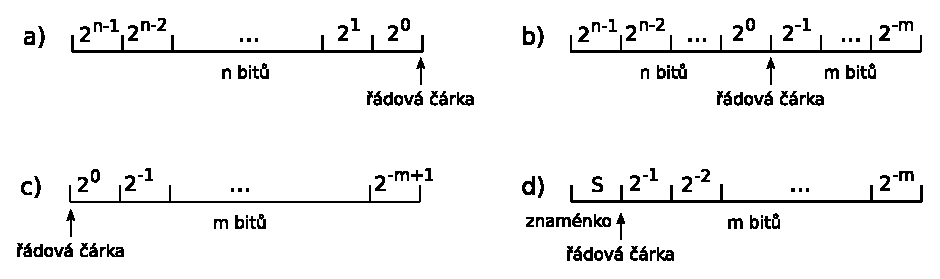
\includegraphics{obrazky/pevna_rad_carka.eps}}
%\caption{Rôzne formáty fixed point aritmetiky \cite{KrausDisP}}
%\label{formatfixpoint}
%\end{figure}
%\bigskip

\begin{figure}[h]
\centering
\subfloat{\label{formatfixpointa} 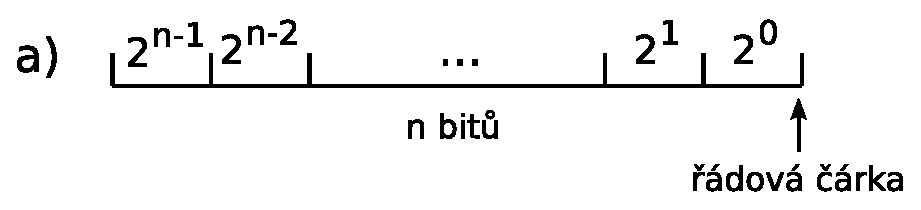
\includegraphics[width=0.44\linewidth]{obrazky/pevna_rad_carkaa.eps}} \hspace{0.6cm}
\subfloat{\label{formatfixpointb} 
\includegraphics[width=0.405\linewidth]{obrazky/pevna_rad_carkab.eps}} \\ \bigskip
\subfloat{\label{formatfixpointc} 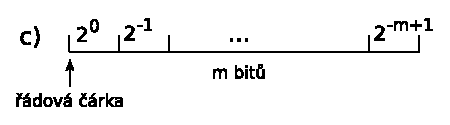
\includegraphics[width=0.405\linewidth]{obrazky/pevna_rad_carkac.eps}} \hspace{1.2cm}
\subfloat{\label{formatfixpointd} 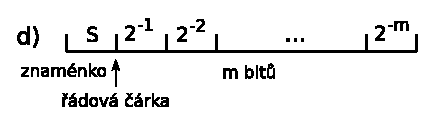
\includegraphics[width=0.405\linewidth]{obrazky/pevna_rad_carkad.eps}}
\caption{Rôzne formáty fixed point aritmetiky \cite{KrausDisP}}
\label{formatfixpoint}
\end{figure}
\bigskip

%Môžme si všimnúť že čísla uložené vo FX sú rovnomerne rozložené na časovej ose.
Vo fixed point aritmetike sa používajú rôzne kódy, napr. priamy kód, doplnkový kód či inverzný kód. V~nasledujúcich kapitolách a pri návrhu integrátorov v~pevnej rádovej čiarke budeme používať doplnkový kód. 

\newpage
\section{Pohyblivá rádová čiarka}
Čísla uložené v~pohyblivej rádovej čiarke sú tvorené exponentom a mantisou. Všeobecný tvar na získanie hodnoty uloženej vo FP je nasledujúci:

\begin{eqnarray}
X = B^{E}\cdot M
\end{eqnarray}

\begin{tabular}{ll}
$ X $ - výsledná hodnota \\
$ B $ - základ sústavy \\
$ E $ - hodnota exponentu \\
$ M $ - mantisa \\
\end{tabular}
\bigskip

Zvýšením počtu bitov v~exponente $ E $ sa zvýši rozsah hodnôt, ktorý je možný reprezentovať, a zvýšením počtu bitov v~mantise $ M $ za zvýši presnosť uložených čísel. Existuje veľa formátov uloženia čísel v~pohyblivej rádovej čiarke. Najpoužívanejší a najrozšírenejší je štandard \textbf{IEEE 754}. Definuje vlastný formát uloženia čísel a viaceré formáty s~rôznou presnosťou. Najpoužívanejšie z~nich sú formáty čísel s~jednoduchou (single) a s~dvojitou (double) presnosťou. Čísla s~jednoduchou presnosťou sú uložené na 32 bitoch, kde MSB je znamienkový bit $ S $, ďalších 8 bitov tvorí exponent $ E $, a zvyšných 23 bitov tvorí mantisu $ M $.

\bigskip
\begin{figure}[h]
\centering
\scalebox{0.2}{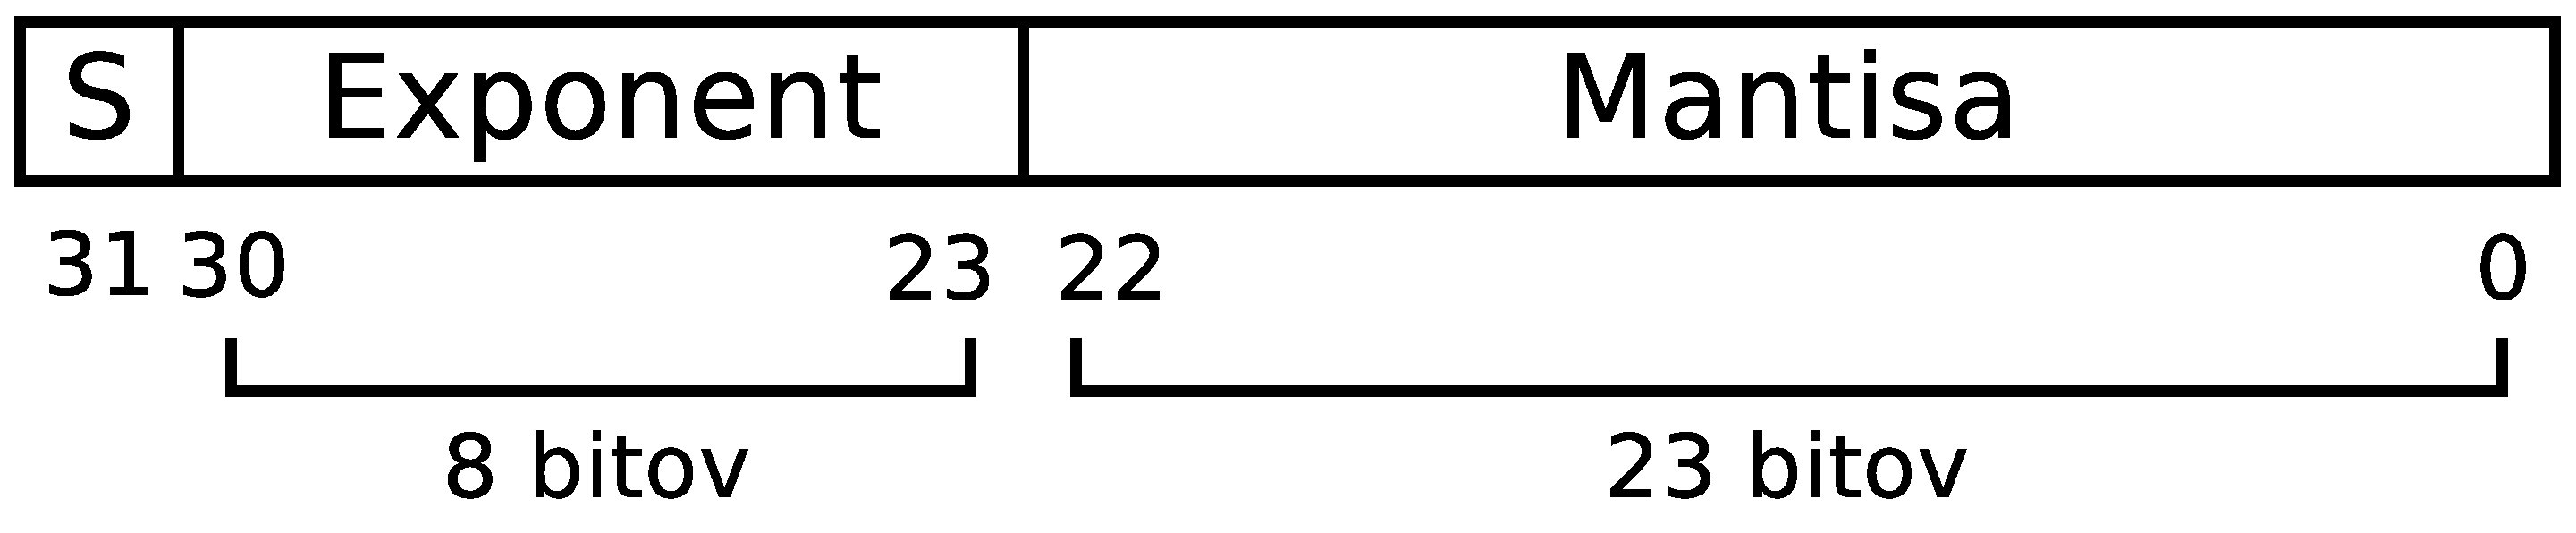
\includegraphics{obrazky/IEEE754_32b.eps}}
\caption{IEEE 754 formát s~jednoduchou presnosťou}
\label{formatFP32}
\end{figure}


Čísla s~dvojitou presnosťou sú uložené v~rovnakom formáte ako čísla s~jednoduchou presnosťou, avšak líšia sa v~počte bitov, ktorý je zväčšený na 64, kde MSB je znamienkový bit $ S $, ďalších 11 bitov tvorí exponent $ E $, a zvyšných 52 bitov tvorí mantisu $ M $.

\bigskip
\begin{figure}[h]
\centering
\scalebox{0.2}{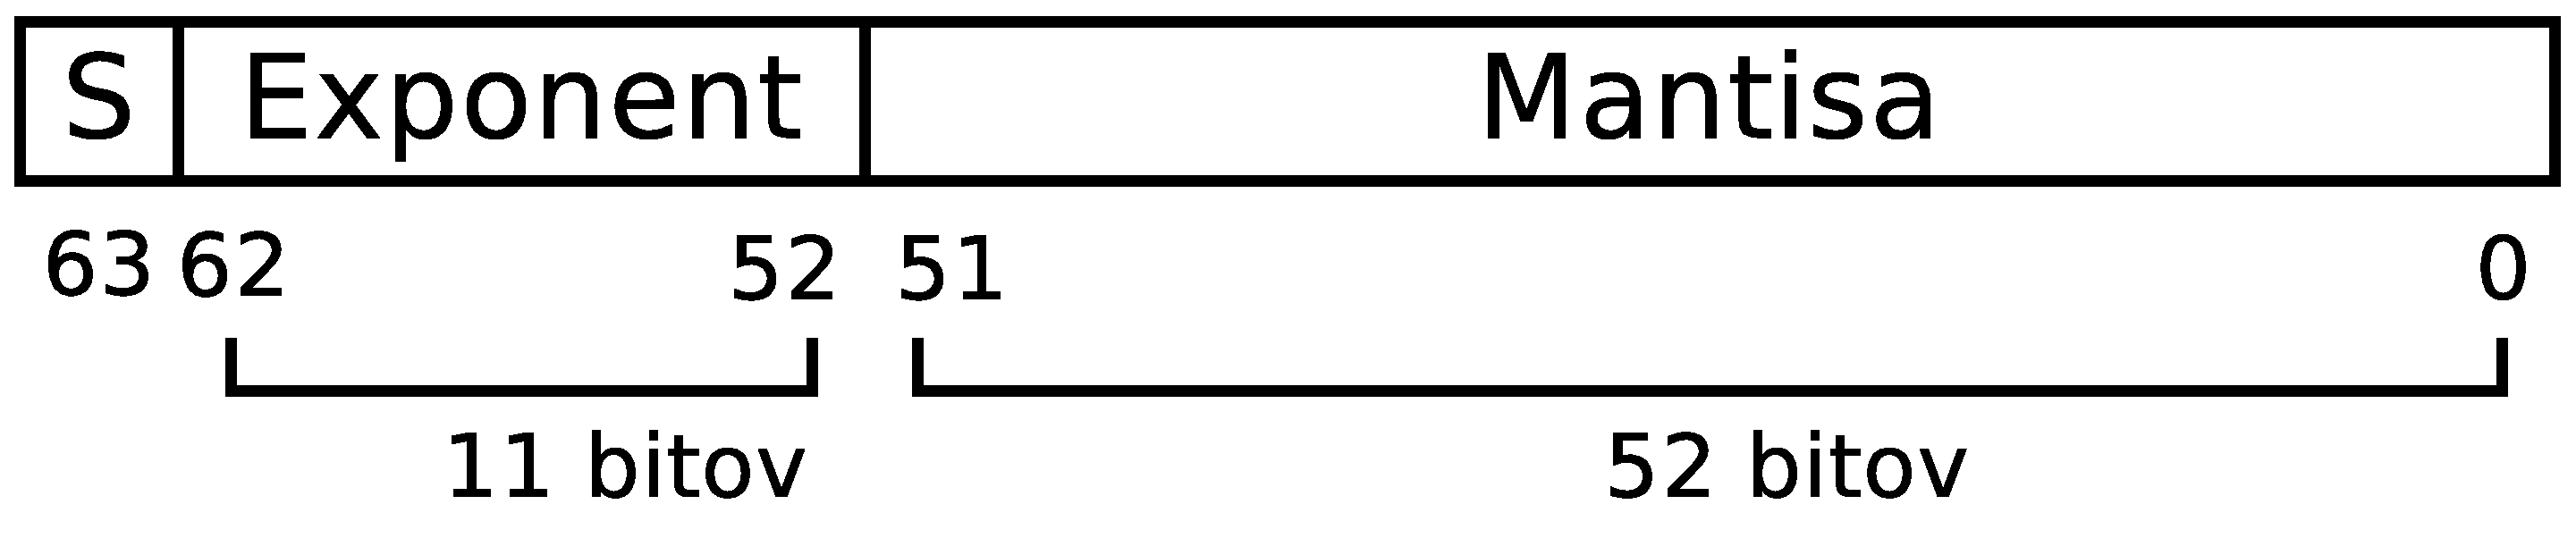
\includegraphics{obrazky/IEEE754_64b.eps}}
\caption{IEEE 754 formát s~dvojitou presnosťou}
\label{formatFP64}
\end{figure}

Znamienko $ S $ nadobúda hodnoty 0, čo značí kladné číslo; alebo 1, čo značí záporné číslo. Exponent je uložený v~kóde s~nepárnym posunutím o~hodnotu BIAS. Táto hodnota je zvolená tak, aby uložený exponent bol vždy kladný. Pri jednoduchej presnosti má teda BIAS hodnotu 127 a pri dvojitej presnosti hodnotu 2047.
\newpage
Hodnota mantisy je uložená v~priamom kóde bez znamienka, znížená o~hodnotu 1, keďže je tu použitá tzv. normalizácia. Mantisa je normalizovaná do tvaru $ 1.M $, kde sa jednotka neukladá -- je skrytá, čím sa ušetrí jeden bit. Hodnotu takto uloženého čísla získame zo vzťahu:

\begin{eqnarray}
X_{754} = -1^{S}\cdot 2^{E-BIAS}\cdot (1,M)
\end{eqnarray}

\begin{tabular}{ll}
$ X_{754} $ - výsledná hodnota \\
$ BIAS $ - 127 alebo 2047 \\
$ E $ - hodnota exponentu \\
$ M $ - mantisa \\
\end{tabular}
\bigskip

Štandard IEEE 754 definuje aj špeciálne hodnoty ako kladnú/zápornú nulu, kladné/záporné nekonečno, či hodnotu NaN (not a number). Tieto hodnoty sú uvedené v~tabuľke~\ref{standard_IEEE754}.
Hodnota mantisy v~normalizovanom tvare je v~intervale $ <1,0; 2,0) $. Ak tomu tak nie je, ide o~tzv. denormalizované číslo, a hodnota exponentu je braná ako $ -126 $. Štandard IEEE 754 definuje aj spôsob vykonávania základných matematických operácií, ktoré sú popísané v~sekciách \ref{PlusMinusFP} a \ref{MulDivFP}.

\bigskip
\begin{table}[h]
\centering
\begin{tabular}{|l|l|l|l|}
\hline
\rowcolor[HTML]{C0C0C0} 
S~(znamienko) & E (exponent) & M (mantisa)       & význam                    \\ \hline
0/1           & 00000000     & nulová hodnota    & +/- 0                     \\ \hline
0/1           & 00000000     & nenulová hodnota  & +/- denormalizované číslo \\ \hline
0/1           & 1 - 254      & ľubovoľná hodnota & +/- FP číslo              \\ \hline
0/1           & 11111111     & nulová hodnota    & +/- $ \infty  $           \\ \hline
0/1           & 11111111     & nenulová hodnota  & NaN                       \\ \hline
\end{tabular}
\caption{Štandard IEEE 754 \cite{FPOnline}}
\label{standard_IEEE754}
\end{table}

\newpage
\subsection{Súčet a rozdiel} \label{PlusMinusFP}
Súčet a rozdiel v~pohyblivej rádovej čiarke sa počíta podľa vzorcov
\begin{eqnarray}
X + Y = (M_{X}\cdot 2^{E_{X} - E_{Y}} + M_{Y})\cdot 2^{E_{Y}} \text{, kde} \quad E_{X} \leq E_{Y} \\
X - Y = (M_{X}\cdot 2^{E_{X} - E_{Y}} - M_{Y})\cdot 2^{E_{Y}} \text{, kde} \quad E_{X} \leq E_{Y}
\end{eqnarray}

Postup výpočtu operácie súčtu/rozdielu v~pohyblivej rádovej čiarke podľa štandardu IEEE 754 (\cite{FPOnline_operacie}, \cite{CamborBP}) je nasledovný:

\begin{enumerate}  
\item Na začiatku výpočtu sa obe čísla skontrolujú na výskyt špeciálnych hodnôt z~tabuľky~\ref{standard_IEEE754}. Ak ide o~špeciálne číslo, výsledok sa určí podľa tabuľky~\ref{special_plus}. Inak sa pokračuje bodom 2.

\item Vykoná sa porovnanie exponetov. Ak sú exponenty rozdielne, mantisu menšieho čísla posunieme o~rozdiel exponentov doprava. Tým docielime rovnosť oboch exponentov. Pri posune je dôležité, aby sme nezabudli na 1, ktorá je skrytá, kvôli normalizácií. Posun sa vykonáva spolu s~toutou 1. 

\item Následne sa porovnajú znamienka, a podľa výsledku sa vykoná sučet alebo rozdiel mantisy väčšieho čísla a posunutej mantisy. Ak došlo k~pretečeniu, mantisa výsledku sa posunie o~jeden bit doprava a hodnota exponentu sa zvýši. Aby bolo možné pretečenie detekovať, je potrebné sčítanie/odčítanie mantís vykonávať na sčítačke o~jeden bit väčšej než je veľkosť mantisy (veľkostou mantisy sa tu myslí počet bitov potrebných na uloženie mantisy aj so skrytou 1, čiže $ |1.M| + 1 $).

\item Ak je to potrebné, vykoná sa normalizácia. Mantisa sa posunie o~potrebný počet bitov doprava resp. doľava, tak, aby bola v~tvare $ 1.M $. O~daný počet bitov sa exponent zvýši resp. zníži.

\item Na koniec výpočtu sa skontroluje hodnota exponentu. Ak je hodnota maximálna, došlo k~pretečeniu výsledku. Ten sa nastaví podľa znamienka na kladné alebo záporné nekonečno. V~opačnom prípade, ak je hodnota exponentu minimálna (nulová), došlo k~podtečeniu, a výsledok je nastavený podľa znamienka na kladnú alebo zápornú nulu.
\end{enumerate}


\begin{table}[h]
\centering
\begin{tabular}{|l|l|l|}
\hline
\rowcolor[HTML]{C0C0C0} 
Hodnota operandu 1 & Hodnota operandu 2 & Výsledok sčítania \\ \hline
FP číslo           & +/- $ \infty $     & +/- $ \infty $    \\ \hline
+/- $ \infty $     & +/- $ \infty $     & +/- $ \infty $    \\ \hline
+ $ \infty $       & - $ \infty $       & NaN               \\ \hline
NaN                & ľubovoľná hodnota  & NaN               \\ \hline
\end{tabular}
\caption{Výsledok operácie sčítania so špeciálnymi hodnotami}
\label{special_plus}
\end{table}

\newpage
\subsection{Násobenie a delenie} \label{MulDivFP}
Násobenie a delenie v~pohyblivej rádovej čiarke sa počíta nasledovne:

\begin{eqnarray}
X \times Y = (M_{X} \cdot M_{Y})\cdot 2^{E_{X} + E_{Y}} \\
X \div Y = ({M_{X}} \div {M_{Y}})\cdot 2^{E_{X} - E_{Y}}
\end{eqnarray}

Postup výpočtu operácií násobenia a delenia podľa štandardu IEEE 754 (\cite{FPOnline_operacie}, \cite{CamborBP}) je nasledovný:

\begin{enumerate}  
\item Rovnako ako pri sčítaný, aj teraz sa na začiatku výpočtu skontroluje výskyt špeciálnych hodnôt oboch čísel podľa tabuľky~\ref{standard_IEEE754}. Ak ide o~špeciálne číslo, výsledok sa určí podľa tabuľky~\ref{special_nasobenie} alebo \ref{special_delenie}. Pri operácii delenia je potrebné kontrolovať nepovolenú operáciu delenie nulou. Pokračuje sa bodom 2.

\item Pri násobení sa hodnota exponentu vypočíta ako súčet exponentov, od ktorého sa odpočíta hodnota \textit{BIAS}. Pri operácii delenia sa hodnota exponentu vypočíta ako rozdiel exponentov, ku ktorému je pripočítaná hodnota \textit{BIAS}.

\item Výsledná mantisa je rovná sučinu resp. podielu mantís. Pri násobení je potrebné použiť násobičku, ktorej bitová šírka sa rovná dvojnásobku počtu bitov mantisy $ 1.M $. Ak dôjde k~pretečeniu alebo k~podtečeniu mantisy, vykoná sa posun mantisy doprava resp. doľava a hodnota exponentu sa zvýši resp. zníži.

\item Pokiaľ je to potrebné, prebehne normalizácia.

\item Na konci výpočtu sa skontroluje hodnota exponentu. Postupuje sa rovnako ako pri operácii súčtu: ak je hodnota exponentu maximálna, nastaví sa podľa znamienka na kladné alebo záporné nekonečno. V~opačnom prípade, ak je hodnota exponentu minimálna (nulová), výsledok sa nastaví podľa znamienka na kladnú alebo zápornú nulu.
\end{enumerate}


\begin{table}[h]
\centering
\begin{tabular}{|l|l|l|}
\hline
\rowcolor[HTML]{C0C0C0} 
Hodnota operandu 1 & Hodnota operandu 2 & Výsledok násobenia \\ \hline
kladné/záporné FP číslo & +/- $ \infty $ & +/- $ \infty $ \\ \hline
nula           & +/- $ \infty $ & NaN \\ \hline
+/- $ \infty $ & +/- $ \infty $ & +/- $ \infty $ \\ \hline
NaN & ľubovoľná hodnota & NaN \\ \hline
\end{tabular}
\caption{Výsledok operácie násobenia so špeciálnymi hodnotami}
\label{special_nasobenie}
\end{table}

\begin{table}[h]
\centering
\begin{tabular}{|l|l|l|}
\hline
\rowcolor[HTML]{C0C0C0} 
Hodnota operandu 1 & Hodnota operandu 2 & Výsledok násobenia \\ \hline
kladné/záporné FP číslo & +/- 0 & +/- $ \infty $ \\ \hline
0 & 0 & NaN \\ \hline
\end{tabular}
\caption{Výsledok operácie delenia so špeciálnymi hodnotami}
\label{special_delenie}
\end{table}

\chapter{Numerické integrátory} \label{NUM_INTEGRATORY}
Numerický integrátor je hardvérový komponent, ktorý slúži na výpočet numerickej integrácie. Podľa spôsobu výpočtu a komunikácie medzi komponentmi integrátora sa numerické integrátory delia na sériové, sériovo-paralelné a paralelné. My sa budeme zaoberať paralelnými numerickými integrátormi, kvôli ich jednoduchosti a rýchlosti výpočtu. Ďalej môžeme numerické integrátory rozdeliť na jednovstupé a dvojvstupé. Jedno vstupý integrátor vykonáva integráciu vstupnej hodnoty a posiela ju na výstup. Schéma integrátora je znázornená na obrázku \ref{schema_i} a ako z názvu vyplýva obsahuje jeden vstup pre vstupnú hodntotu. Ďalej obsahuje jeden vstup pre počiatočnú podmienku a jeden výstup pre výsledok výpočtu. Dvojvstupové integrátory obsahujú jeden vstup pre počiatočnú podmienku, dva vstupy pre prívod operandov a jeden výstup pre výsledok výpočtu. Schéma integrátora je znázornená na obrázku \ref{schema_ndi}. Tieto integrátory rozdeľujeme podľa použitej operácie na násobiace a deliace integrátory.

V nasledujúcich podkapitolách predstavíme jednotlivé návrhy paralelných násobiacich a paralelných deliacich integrátorov, oba typy v pevnej a v pohyblivej rádovej čiarke. Predstvíme taktiež jednovstupý paralelný integrátor v pohyblivéj rádovej čiarke.
\bigskip


\begin{figure}[h]
\centering
\subfloat[Schéma jednovstupého integrátora]{\label{schema_i} 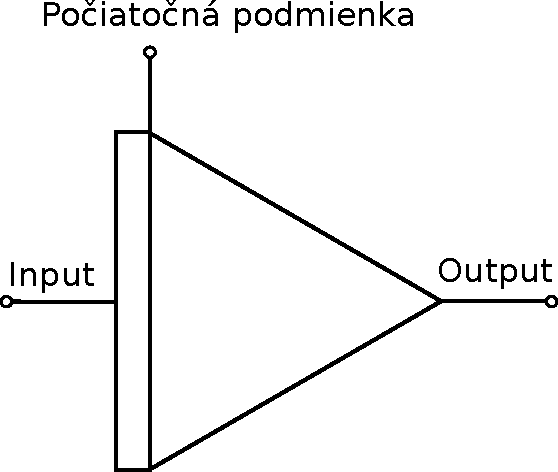
\includegraphics[width=0.4\linewidth]{obrazky/jednoduchy_integrator.pdf}} \hspace{1.0cm}
\subfloat[Schéma dvojvstupého násobiaceho/deliaceho integrátora]{\label{schema_ndi} 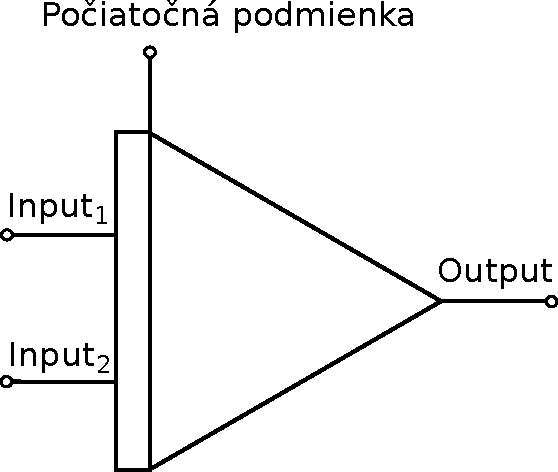
\includegraphics[width=0.4\linewidth]{obrazky/del_nas_integrator.pdf}}
\label{schema_i_ndi}
\caption{Schéma jendovstupého a dvojvstupého integrátora}
\end{figure}



\section{Násobiaci integrátor v~pevnej rádovej čiarke}
Násobiaci integrátor počíta rovnicu \eqref{dif_nasobenie} pomocou \eqref{DY1_cleny_nasobenia} -- \eqref{DY4_cleny_nasobenia}. Na základe týchto rovníc bol vytvorený návrh paralelného násobiacého integrátora, ktorý je na obrázku~\ref{ppni}. Návrh vychádza z~práce V. Závadu \cite{ZavadaBP} a bol upravený a rozšírený o~počet registrov $ DRn $ a $ DQn $, ktoré slúžia na ukladanie prichádzajúcich členov. Počet týchto registorov je stanovený podľa použitej aritmetiky a použadvanej presnosti.

Každý člen $ DYn $ obsahuje postupné delenie integračného kroku $ h $. Tieto hodnoty sú predpočítané a uložené v~sade registrov $ h $. Avšak nie je potrebné uložiť všetkých 20 hodnôt, stačí uložiť len tie hodnoty, ktorých deliteľ je nepárne číslo. Ostatné hodnoty je možné vypočítať jednoduchým posunom registra doprava, čo je vlastne delenie číslom 2. Týmto spôsobom znížime počet registrov o~polovicu. Počet operácií potrebných na výpočet sa nezvýši, keďže posun registra je možné vykonávať v~predstihu a paralelne s~inými operáciami.

\bigskip
\begin{figure}[h]
\centering
\scalebox{0.6}{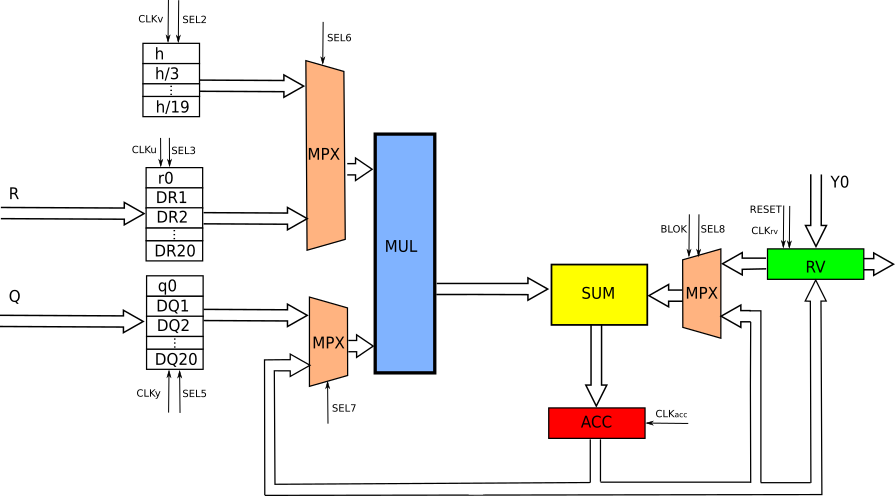
\includegraphics{obrazky/ppni_fx20.png}}
\caption{Paralelno-paralelný násobiaci integrátor \cite{ZavadaBP}}
\label{ppni}
\end{figure}

Na začiatku výpočtu sú pomocou signálu \textit{RESET} vynulované všetky registre, a nastavia sa potrebné signály na multiplexory \textit{MPX}. Následne je do registra \textit{RV} nahraná počiatočná podmienka, do registra \textit{h} je nahraný integračný krok metódy a do registrov \textit{h/i, i=3,5..19} sú nahrané predpočítané konštanty. Po prijatí hodnôt \textit{R} a \textit{Q} sa začne výpočet. Výsledok výpočtu je uložený v~registri \textit{RV}.


\section{Deliaci integrátor v~pevnej rádovej čiarke}
Tento integrátor počíta rovnicu \eqref{dif_delenie} pomocou členov \eqref{DY1_cleny_delenia} - \eqref{DY4_cleny_delenia}. Podobne, ako u~násobiaceho integrátora, bol z~týchto rovníc vytvorený návrh paralelného deliaceho integrátora. Návrh vychádza z~bakalárskej práce \cite{MatecnyBP} a bol upravený podobne ako predošlí násobiaci integrátor zvýšením počtu registrov $ DUn $ a $ DVn $. Taktiež sa zvýšil počet registrov $ DYn $, ktoré slúžia na uloženie jednotlivých členov Taylorovej rady, kedže na výpočet nasledujúceho člena je použitý predchádzajúci člen. Deliaci integrátor, narozdiel od násobiaceho integrátora, nepoužíva sadu registrov $ h $, ale podobnú sadu registrov, ktorá obsahuje hodnoty $ 1/n $. Podobne ako u~násobiaceho integrátora je možné zmenšiť počet týchto registrov na polovicu s~využitím operácie \textit{shift}. Register \textit{const} obsahuje \textit{counter}, ktorý sa postupne inkrementuje, a s~ktorým sa násobí hodnota $ DYn $. Výsledná hodnota je uložená do daného registra $ DYn $ a znova použitá v~ďalšom výpočte, čím sa ušetrí operácia násobenia.

\begin{figure}[h]
\centering
\scalebox{0.5}{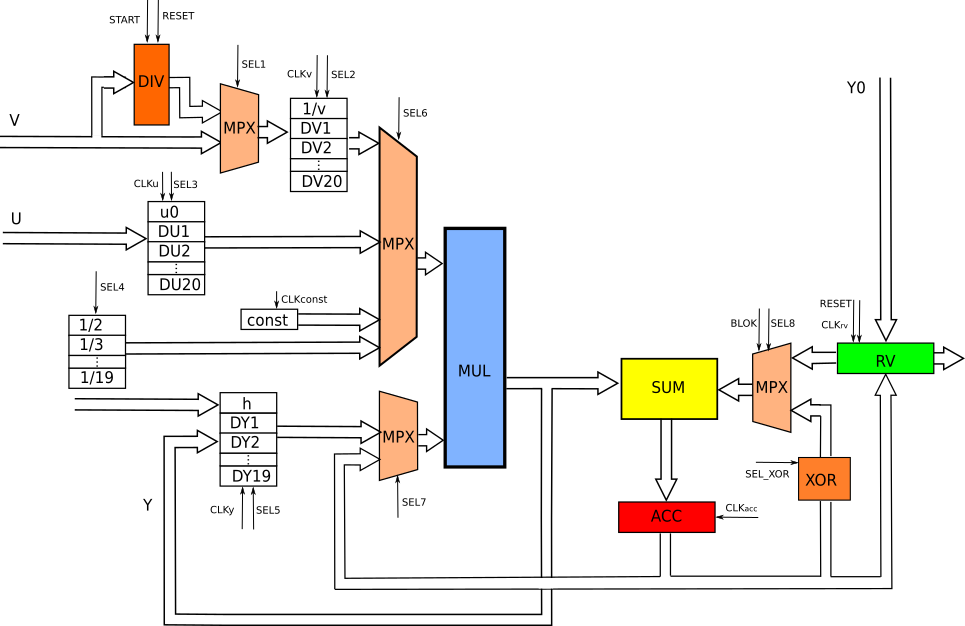
\includegraphics{obrazky/ppdi_fx20.png}}
\caption{Paralelno-paralelný deliaci integrátor \cite{MatecnyBP}}
\label{ppdi}
\end{figure}
\bigskip

Podobne ako pri násobiacom integrátore, aj pri paralelnom deliacom integrátore sú na začiatku výpočtu vynulované registre pomocou signálu \textit{RESET} a nastavené signály multiplexorov \textit{MPX}. Ďalej je do registra \textit{RV} nahraná počiatočná podmienka a do registra $ h $ je nahraný integračný krok. Do registrov $ 1/n $ sú uložené predpočítané konštanty. Po prijatí hodnôt $ U $ a $ V $ sa začne výpočet. Hodnota $ V $ je privedená do deličky $ DIV $ a spustí sa výpočet $ 1/v $ s~použitím deliaceho algoritmu \textit{SRT}. Delenie je realizované len raz počas celého výpočtu, keďže ide o~veľmi náročnú operáciu. Kvôli optimalizácii je paralelne s~delením realizovaný výpočet násobenia $ uh $.
Po skončení výpočtu je výsledok uložený do registra $ RV $. 

\newpage
\section{Jendovstupý integrátor v pohyblivéj rádovej čiarke}
Tento integrátor bol navrhnutý podľa rovníc \eqref{DY_cleny} na zálade ktorých počíta difernciálnu rovnucu \eqref{jednoducha_rovnica}. Z toho vyplýva, že vykonáva numerickú integráciu vstupnej hodnoty a následne výslednú hodnotu posiela na výstup. Na naštartovanie výpočtu slúži počiatočna podmienka. Tá je nahraná na začiatku výpočtu do registra RV.RD.
Schéma integrátora je na obrázku \ref{ppi_fp} a vychádza z práce J. Opálku \cite{OpalkaBP}.

\bigskip
\begin{figure}[h]
\centering
\scalebox{0.4}{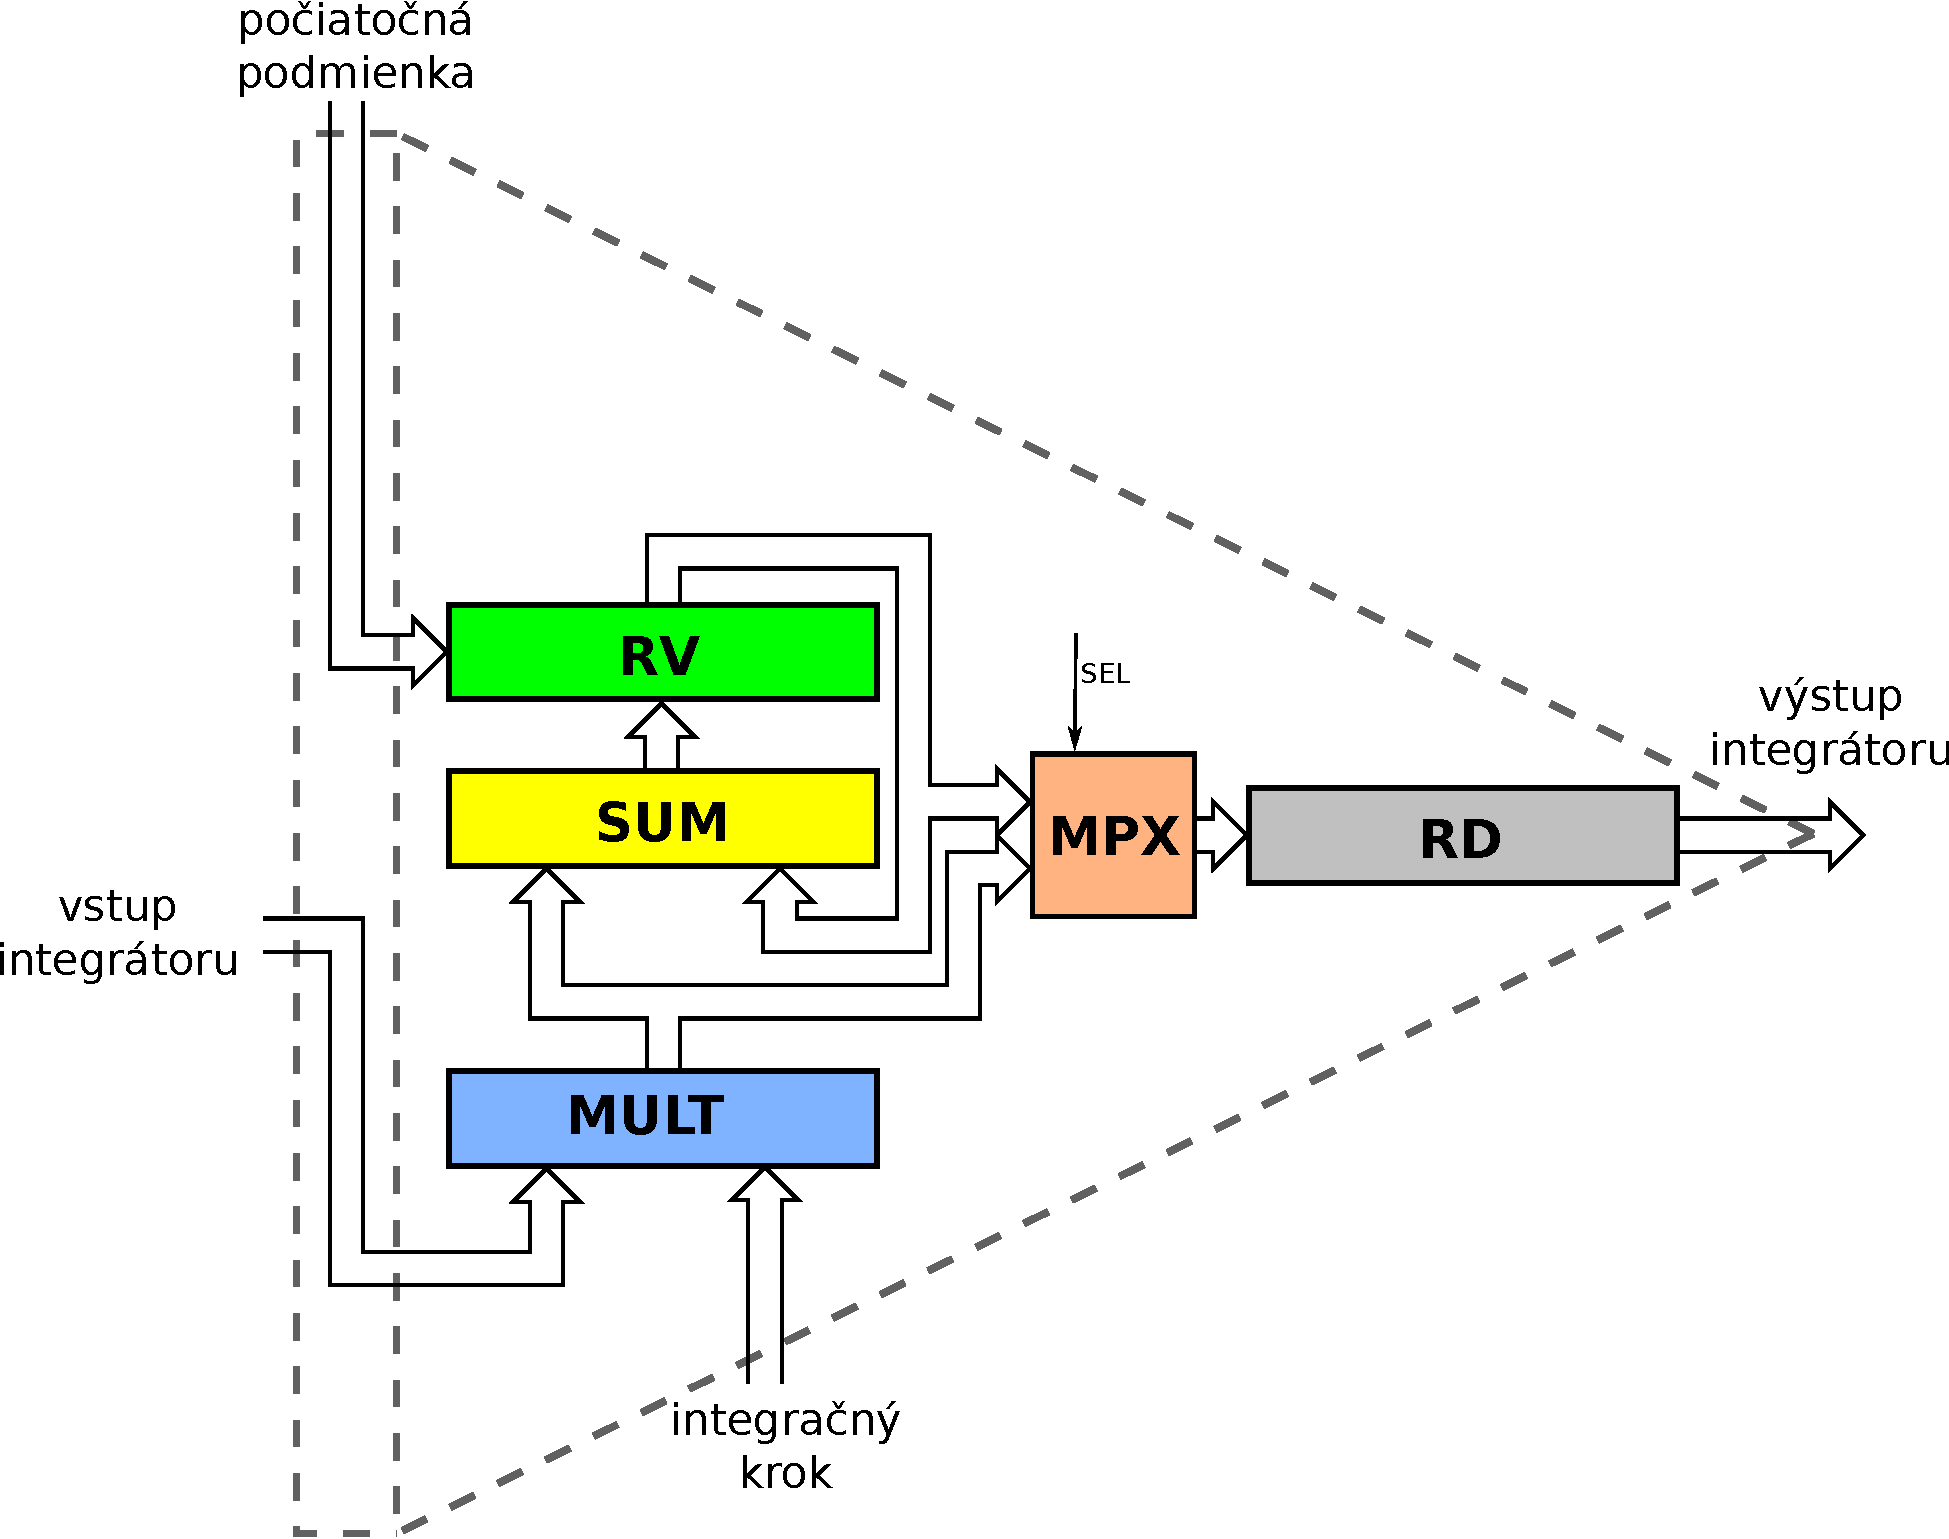
\includegraphics{obrazky/integrator_paralelny.pdf}}
\caption{Paralelný jednovstupový integrátor v pohyblivej rádovej čiarke}
\label{ppi_fp}
\end{figure}
\bigskip

\section{Násobiaci integrátor v~pohyblivej rádovej čiarke}
Blokové schémy zapojenia integrátorov pracujúcich v~pohyblivej rádovej čiarke vychádzajú z~predchádzajúcich návrhov, ale boli rozšírené o~prácu so znamienkami, s~mantisou a s~exponentmi. Samotný výpočet exponenta sa deje v~komponente \textit{EXP}, ktorého návrh je zobrazený na obrázku~\ref{ppi_fp_exp}.

\bigskip
\begin{figure}[h]
\centering
\scalebox{0.8}{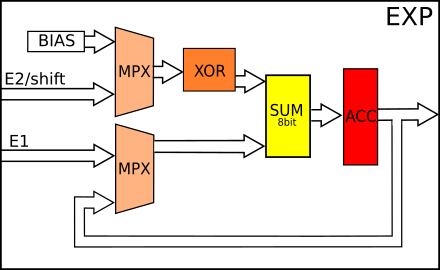
\includegraphics{obrazky/ppdi_fp_exp.png}}
\caption{EXP - blok pracujúci s~exponentmi}
\label{ppi_fp_exp}
\end{figure}
\bigskip

Komponent \textit{EXP} slúži na vykonávanie výpočtov s~exponentmi, ktoré sú popísané v~sekciách~\ref{PlusMinusFP} a~\ref{MulDivFP}. Obsahuje dva vstupy, do ktorých sú privedené jednotlivé exponenty z~komponentov $ DIV $, $ MUL $ a $ SUM $. Výpočet sa uskutočňuje pomocou paralelnej sčítačky na 8 alebo 11 bitoch, podľa v~závislosti použitej aritmetiky.
Pri vykonávaní operácie súčinu alebo rozdielu slúži komponent \textit{EXP} na výpočet rozdielu exponentov. Výsledná hodnota rozdielu je privedená naspäť do sčítačky \textit{SUM} cez register \textit{ACC}.
Pri operácii násobenia alebo delenia slúži komponent \textit{EXP} na výpočet výsledného exponentu. Podľa typu operácie sa vykoná sučet alebo rozdiel prijatých exponentov. Táto hodnota je uložená v~registri \textit{ACC} a privedená naspäť do sčítačky $ SUM_{8bit} $ s~hodnotou z~registra $ BIAS $. Vykoná sa súčet alebo rozdiel týchto hodnôt a výsledná hodnota je privedená naspäť do násobičky $ MUL $ alebo deličky $ DIV $.
Okrem spomenutých operácií slúži komponent $ EXP $ na zvýšenie alebo zníženie hodnoty exponenta na základe posunu mantisy pri pretečení/podtečení a pri normalizácii.

Kvôli prehľadnosti neobsahuje schéma zapojenia  znázornenie výpočtu znamienka a rozdelenie operandov na znamienko, exponent a na mantisu, a ich opätovné zloženie. Tieto oberácie sa vykonávajú v~komponentoch \textit{DIV}, \textit{MUL} a \textit{SUM}.\\

Návrh paraleného násobiaceho integrátora v~pohyblivej rádovej čiarke je na obrázku~\ref{ppni}. Čísla v~pohyblivej rádovej čiarke môžeme zobraziť presnejšie ako čísla v~pevnej rádovej čiarke, čiže pri uložení malých čísel v~pohyblivej rádovej čiarke dochádza k~menšej zaokrúhľovacej chybe. Z~tohto dôvodu je možné počítať Taylorovu radu s~použitím väčšieho počtu členov a zvýšiť tak presnoť výpočtu. Inegrátory v~pohyblivej rádovej čiarke sú teda navrhnuté tak, aby umožňovali výpočet až na 40 členov Taylorovej rady. Kvôli tomu, ako môžeme vidieť v~návrhu, je zvýšený počet registrov $ DRn $ a $ DQn $ na 40. Sada registrov $ h/i, i=3,5..39 $ obsahuje 20 registrov, kde sú zvyšné hodnoty dopočítané rovnako ako pri integrátoroch v~pevnej rádovej čiarke.

\begin{figure}[h]
\centering
\scalebox{0.6}{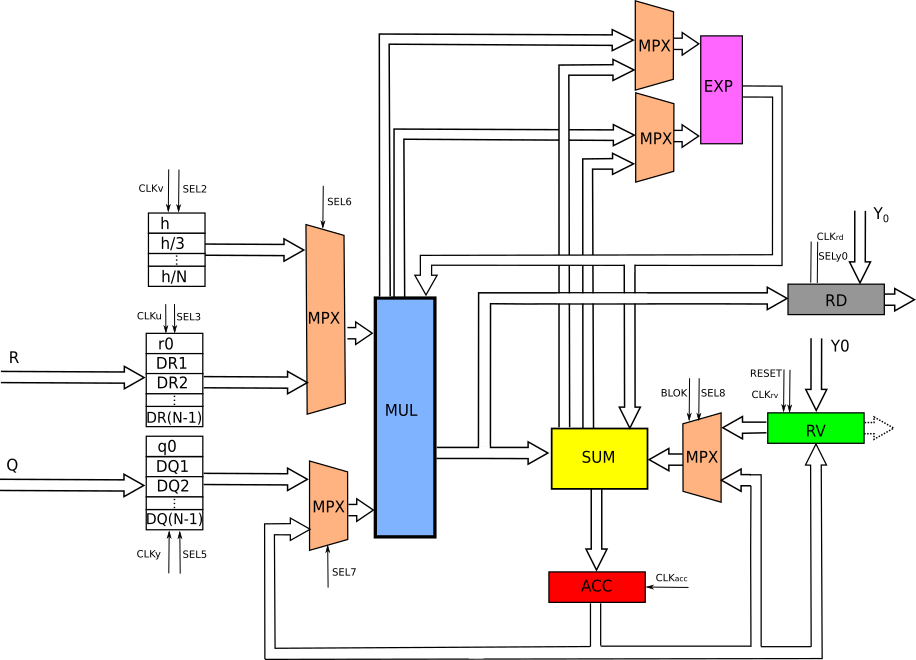
\includegraphics{obrazky/ppni_fp40.png}}
\caption{Paralelno-paralelný násobiaci integrátor v~pohyblivej rádovej čiarke}
\label{ppni_fp}
\end{figure}
\bigskip

Spôsob výpočtu paralelného násobiaceho integrátora v~pohyblivej rádovej čiarke je rovnaký ako pri násobiacom integrátore v~pevnej rádovej čiarke. Rozdielne sa vykonávajú operácie násobenia a sčítania. Po privedení hodnôt na vstupy násobičky $ MUL $ alebo sčítačky $ SUM $ sú čísla v~FP uložené do pomocných registrov v~týchto komponentoch. Z~týchto registrov sú jednotlivé časti FP čísla rozdistribuované do samostatných výpočetných obvodov. Znamienka sú privedené ku komponentu $ XOR $, ktorý vykonáva nonekvivalenciu. Exponenty, ako je popísané vyššie, spracúva komponent $ EXP $. Mantisy sú privedené do paralelnej násobičky alebo sčítačky. Výsledné hodnoty sú uložené do výstupného registra daného komponentu ($ MUL $ alebo $ SUM $) a poskytnuté na jeho výstupe k~ďalšiemu výpočtu.

\section{Deliaci integrátor v~pohyblivej rádovej čiarke}
Paralelný deliaci integrátor v~pohyblivej rádovej čiarke je najzložitejší z~navrhnutých integrátorov. Obsahuje všetky spomínané operácie: sčítanie, odčítanie, násobenie a delenie; a všetky vykonáva v~pohyblivej rádovej čiarke.
Operácie násobenia a sčítania sa vykonávajú rovnako ako v~paralelnom násobiacom integrátore v~pohyblivej rádovej čiarke. Operácia delenia sa vykonáva iba raz za celý výpočet a to paralelne s~operáciou násobenia, ako je tomu aj v~deliacom interátore v~FX aritmetikou. Tu však môže dôjsť ku kolízii v~použití komponentu $ EXP $. Keďže delenie je náročnou operáciou a jej vykonávanie je zdĺhavé, komponent $ EXP $ je poskytnutý najskôr na výpočet exponentov pri operácii násobenia. Po uvoľnení komponentu $ EXP $ násobičkou $ MUL $ je komponent $ EXP $ pridelený deličke $ DIV $ na výpočet exponentov. Po skončení delenia je podiel uložený do registra $ 1/v $ a pokračuje sa v~ďalšom výpočte.


\begin{figure}[h]
\centering
\scalebox{0.55}{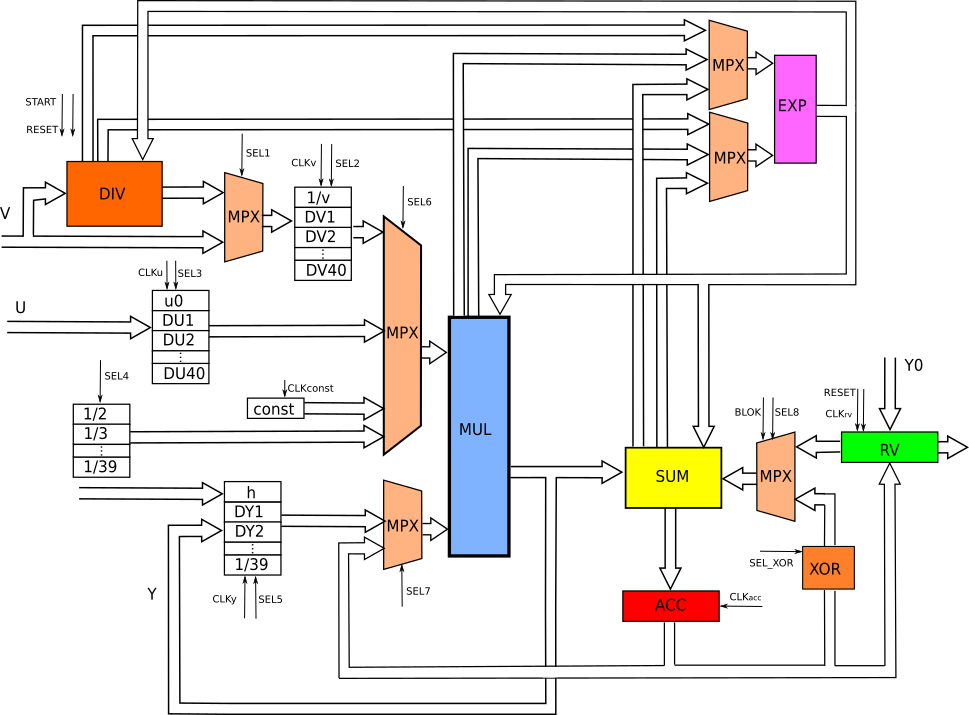
\includegraphics{obrazky/ppdi_fp40.png}}
\caption{Paralelno-paralelný deliaci integrátor v~pohyblivej rádovej čiarke}
\label{ppdi_fp}
\end{figure}
\bigskip

\newpage
\section{Sústava diferenciálnych rovníc}
Integrátory, ktoré sme si popísali je možné medzi sebou zapojiť a riešiť tak diferenciálnu rovnicu. Po zapojení integrátorov nebude nutné predpočítavať vstupné hodnoty, ale stačí zadať počiatočné podmienky na naštartovanie výpočtu a všetky ostatné hodnoty sa dopočítajú.
Zvoľme konkrétnu diferenciálnu rovnciu s operáciou násobenia v tvare:
\begin{eqnarray}
y' & = & sin(t) e^{-t} \, , \quad y(0) = 1 \label{dif_sint_et}
\end{eqnarray}
\bigskip

Rovnicu prevedieme do sústavy diferenciálnych rovníc:
\begin{eqnarray}
y' & = & qr \, , \quad y(0) = 1 \nonumber \\
r' & = & -r \, , \quad r(0) = 1 \nonumber \\
q' & = & s \, , \quad q(0) = 0 \nonumber \\
s' & = & -q \, , \quad s(0) = 1 \nonumber \\
\end{eqnarray}

Zo sústavy rovníc vytvoríme schcému zapojenia integrátorov znázornenú na obrázku \ref{ppi_fp_sustava}. Zo schémy zapojenia je možné následne vytvoriť vhdl kód a vykonať výpočet na fpga. Takýto postup je vhodný pre rozsiahle diferenciálne rovnice s väčším počtom operácií, ktorých výpočet by bol vykonávaný veľmi často. Vhodnejší spôsob použitia sa ponúka prepojovacia sieť medzi rôznimy integrátormi. Pred výpočtom by sa sieť nakonfigurovala podľa danej diferenciálnej rovnice a výpočet by mohol prebiehať bez nutnosti syntézy. Táto varianta je síce priestorovo náročná, ale ponúka variabilitu výpočtu. V ďalšej kapitole si predstavíme implementáciu popísaných integrátorov a taktiež implementáciu sústavy diferenciálnch rovníc pomocou metódy bez použitia prepojovacej siete.
\bigskip

\begin{figure}[h]
\centering
\scalebox{0.5}{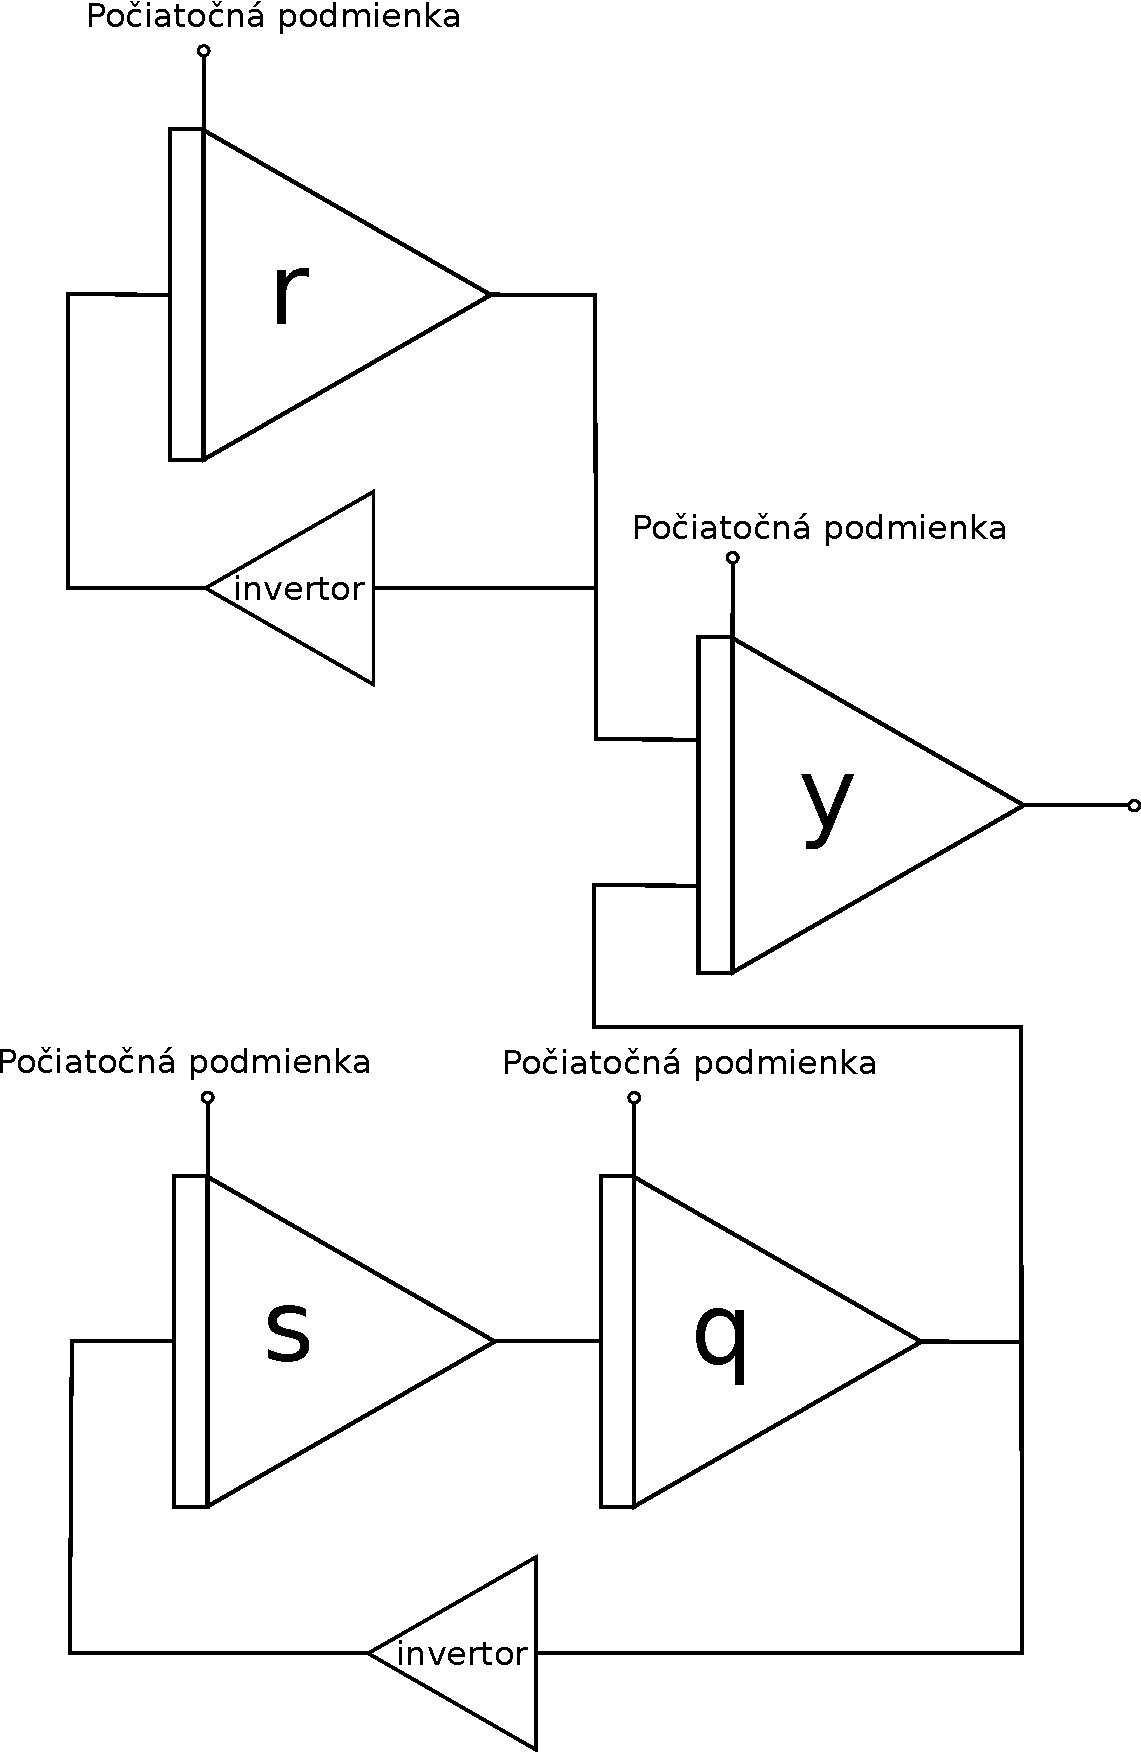
\includegraphics{obrazky/sustava_integratorov.pdf}}
\caption{Schéma zapojenia integrátorov \cite{MatecnyBP}}
\label{ppi_fp_sustava}
\end{figure}
\bigskip


\chapter{Implementácia integrátorv vo VHDL}
Jednotlivé integrítory boli implementované v prostredí Xilinx ISE a následne odsimulované v Model Sim požitím testbanchu.

\section{Integrátory vo pevnej rádovej čiarke}
Paralelný dvojvstupový násobiaci integrátor vo fixpoint aritmetike bol implementovaný v dvoch verziách a to na 32 a 64 bitoch. Veľkosť použitej aritmetiky je však možné jednoducho zväžšiť keďže celý kód je písaný genericky. Taktiež je možné zmeniť počet cyklov výpočtu, čiže počet počítaných členov Taylorovej rady, avšak v závislosti od počtu cyklov je nutné upraviť aj počet registrov h/i kde i >= 2.
Pre 32 bitovú verziu bola použitá FX aritmetika s jedným znamienkovým bitov, xx bitami pred desatinnou čiatkou a xx bitmi za desatinou čiarkou. Výpočet počíta s Taylorovou metódou xx rádu a teda pri výpočte sa počíta x členov Taylorovej rady. 
Podobne 64 bitová verzia pracuje s aritmetikou s jedným znaminekovým bitom, xx bitmi pred desatinou čiarkou a xx bitmi za desatinou čiarkou. V tejto verzií sa počíta Taylorova rada xx. rádu. 

Paralelný delaici integrátor vo fixpoint arimtmetike bol implementovaný podobne ako násobiaci integrátor.


\section{Integrátory v pohyblivej rádovej čiarke}
Jednovstupový integrátor v pohyblivéj rádovej čiarke bol implmentovaný v 32 a v 64 bitovej verzií. Počet cyklov výpočtu nie je stanovený v implementácií integrátra ako to je u dvojvstupových integrotoroch, kedže integrátor vykonáva jednoduchú integráciu a pri výpočte nepotrebuje ukladať všetky predchádzajúce členy. Je ovládaný len pomocou signálov RESET a EN. Tie určujú či sa výpočet začína od začiatku alebo sa pokračuje výpočtom ďalšieho člena. Honoty kroku h a jeho podielov nie sú uložené v komponent eintegrátora, ale sú privádzané z nadradenej komonenty. Dôvodom je redukovanie duplicity registrov. Podrobnejšie vysvetlenie nájdeme v kapitole \ref{impl_rovnice}.


Násobiaci a deliaci integrátor v pohyblivéj rádovej čiarke boli taktiež implementované vo verziách s 32 a 64 bitmi. Integrátory obsahujú paralelnú FP násobičku, paralelnú FP deličku a paralelnú FP sčítačku. Všetky komponenty boli prezvaté z xx a následne upravené a optimalizované pre daný výpočet. Komponenty vykonávajú operácie sčítanie, násobenia a delenie v troch hodinovcýh taktoch. Pri výpočte 

\section{Sústava integrátorv}

Naprogramovanie FPGA VRTEX-5. Pre zložitú prácu a neúspešné sprevádzkovanie displeja, prípadne iných výstupných metód, boli integrátory naprogramované a otestované v FPGA Spartan na prípravku Fitkit.


\chapter{Analýza}
\section{Porovanie Taylorovej rady s metódou Runge-Kutta 2. radu}
\section{Porovanie Taylorovej rady s metódou Runge-Kutta 4. radu}

\chapter{Záver}
V~tejto práci sme sa zaoberali numerickou integráciou pomocou metódy Taylorovej rady. Úpravou jej členov sme získali potrebné rovnice, z~ktorých boli vytvorené jednotlivé návrhy integrátorov.
Rozšírili sme návrhy paralelných integrátorov s~operáciou násobenia a delenia v~pevnej rádovej čiarke tak, aby s~nimi bolo možné počítať diferenciálne rovnice na 20 členov Taylorovej rady. Ďalej sme tieto integrátory navrhli aj v~prevedení pohyblivej rádovej čiarky. Navrhli sme komponent slúžiaci na výpočet exponentu a na jeho úpravu pri normalizácii. Keďže výpočet v~aritmetike pohyblivej rádovej čiarky je presnejší, integrátory využívajúce túto aritmetiku sú navrhnuté na riešenie diferenciálnych rovníc až na 40 členov Taylorovej rady.

Ďalším pokračovaním práce je popísanie navrhnutých integrátorov vo VHDL, otestovanie ich funkčnosti na VIRTEX5 a následné analyzovanie ich časovej a priestorovej zložitosti v~porovnaní s~metódou Runge-Kutta.

%=========================================================================

  
  % Kompilace po částech (viz výše, nutno odkomentovat)
  % Compilation piecewise (see above, it is necessary to uncomment it)
  %\subfile{projekt-01-uvod-introduction}
  % ...
  %\subfile{chapters/projekt-05-conclusion}


  % Pouzita literatura / Bibliography
  % ----------------------------------------------
\ifslovak
  \makeatletter
  \def\@openbib@code{\addcontentsline{toc}{chapter}{Literatúra}}
  \makeatother
  \bibliographystyle{bib-styles/czechiso}
\else
  \ifczech
    \makeatletter
    \def\@openbib@code{\addcontentsline{toc}{chapter}{Literatura}}
    \makeatother
    \bibliographystyle{bib-styles/czechiso}
  \else 
    \makeatletter
    \def\@openbib@code{\addcontentsline{toc}{chapter}{Bibliography}}
    \makeatother
    \bibliographystyle{bib-styles/englishiso}
  %  \bibliographystyle{alpha}
  \fi
\fi
  \begin{flushleft}
  \bibliography{projekt-20-literatura-bibliography}
  \end{flushleft}

  % vynechani stranky v oboustrannem rezimu
  % Skip the page in the two-sided mode
  \iftwoside
    \cleardoublepage
  \fi

  % Prilohy / Appendices
  % ---------------------------------------------
  \appendix
\ifczech
  \renewcommand{\appendixpagename}{Přílohy}
  \renewcommand{\appendixtocname}{Přílohy}
  \renewcommand{\appendixname}{Příloha}
\fi
\ifslovak
  \renewcommand{\appendixpagename}{Prílohy}
  \renewcommand{\appendixtocname}{Prílohy}
  \renewcommand{\appendixname}{Príloha}
\fi
%  \appendixpage

% vynechani stranky v oboustrannem rezimu
% Skip the page in the two-sided mode
%\iftwoside
%  \cleardoublepage
%\fi
  
\ifslovak
%  \section*{Zoznam príloh}
%  \addcontentsline{toc}{section}{Zoznam príloh}
\else
  \ifczech
%    \section*{Seznam příloh}
%    \addcontentsline{toc}{section}{Seznam příloh}
  \else
%    \section*{List of Appendices}
%    \addcontentsline{toc}{section}{List of Appendices}
  \fi
\fi
  \startcontents[chapters]
  \setlength{\parskip}{0pt}
  % seznam příloh / list of appendices
  % \printcontents[chapters]{l}{0}{\setcounter{tocdepth}{2}}
  
  \ifODSAZ
    \setlength{\parskip}{0.5\bigskipamount}
  \else
    \setlength{\parskip}{0pt}
  \fi
  
  % vynechani stranky v oboustrannem rezimu
  \iftwoside
    \cleardoublepage
  \fi
  
  % Přílohy / Appendices
  % Tento soubor nahraďte vlastním souborem s přílohami (nadpisy níže jsou pouze pro příklad)
% This file should be replaced with your file with an appendices (headings below are examples only)

% Umístění obsahu paměťového média do příloh je vhodné konzultovat s vedoucím
% Placing of table of contents of the memory media here should be consulted with a supervisor
%\chapter{Obsah priloženého paměťového média}

\chapter{Obsah CD}

Priložené CD obsahuje:\\
\begin{itemize}
\item Text tejto práce vo formáte Pdf.
\item Zdrojové súbory tejto práce v \LaTeX u.
\item Zdrojové súbory VHDL paralelného deliaceho integrátora.
TODO dopisať
\end{itemize}


%\chapter{Manuál}

%\chapter{Konfigurační soubor} % Configuration file

%\chapter{RelaxNG Schéma konfiguračního souboru} % Scheme of RelaxNG configuration file

%\chapter{Plakát} % poster





%\chapter{Riešenie rôznych typov diferenciálnych rovníc}
%
%\subsection{Riešenie diferenciálnej rovnice s~operáciou násobenia} \label{priloha_nasobenie}
%Předpokládejme zadanou obecnou diferenciální rovnici se zadanou počáteční podmínkou:
%\begin{equation}
%\label{nasobeni_integrace}
%y'= q \cdot r~,~~~~~~y(0)=y_0
%\end{equation}
%
%Pro každou proměnnou v~rovnici je potřeba vytvořit Taylorovu řadu. Taylorovy řady pro zadanou rovnici vypadají následovně:
%\begin{eqnarray}
%y_{i+1} = DY0_i + DY1_i + DY2_i + DY3_i + \cdots + DY(n)_i\\
%q_{i+1} = DQ0_i + DQ1_i + DQ2_i + DQ3_i + \cdots + QZ(n)_i\\
%r_{i+1} = DR0_i + DR1_i + DR2_i + DR3_i + \cdots + DR(n)_i
%\end{eqnarray}
%
%Výpočet Taylorovy řady pro rovnici součinu se počítá následujícím způsobem:\\\\
%Nultý člen Taylorovy řady je roven počáteční podmínce:
%\begin{equation}
%DY0 = y_0
%\end{equation}
%
%Vyjádření prvního členu Taylorovy řady je následující:
%\begin{equation}
%DY1 = h \cdot y' 
%\end{equation}
%Podle vztahu (\ref{nasobeni_integrace}) je $y'$ na hrazen vztahem $q \cdot r$:
%\begin{equation}
%\label{h*q*r}
%DY1 = h \cdot q \cdot r
%\end{equation}
%
%
%Zderivujeme počáteční funkci (\ref{nasobeni_integrace}) a dostaneme vztah: 
%\begin{equation}
%y'' = q' \cdot r + q \cdot r'
%\end{equation}
%
%Nahradíme derivace pomocí prvků Taylorovy řady.
%\begin{equation}
%DY2 = \frac{h^2}{2!} \cdot ( \frac{DQ1}{h} \cdot r + q \cdot \frac{DR1}{h})
%\end{equation}
%
%Obdobně postupujeme u~třetího prvku další derivací funkce:
%\begin{equation}
%y''' = q'' \cdot r + 2 \cdot q' \cdot r' + q \cdot r''
%\end{equation}
%
%Opět nahradíme derivace členy Taylorovy řady a vyjádříme třetí člen:
%\begin{equation}
%DY3 = \frac{h^3}{3!} (\frac{DQ2}{\frac{h^2}{2!}} \cdot r + 2 \cdot \frac{DQ1}{h} \cdot \frac{DR1}{h} + q \cdot \frac{DR2}{\frac{h^2}{2!}})
%\end{equation}
%\\
%Obdobně postupujeme při vyjadřování dalších členů.
%Jednotlivé členy lze následně upravit pokrácením. Zde jsou uvedeny první čtyři členy:
%\begin{eqnarray}
%DY1 &=& h \cdot q \cdot r\\
%DY2 &=& \frac{h}{2} \cdot ( DQ1 \cdot DR0 + DQ0 \cdot DR1)\\
%DY3 &=& \frac{h}{3} ( DQ2 \cdot DR0 + DQ1 \cdot DR1 + DQ0 \cdot DR2)\\
%DY4 &=& \frac{h}{4} (DQ3 \cdot DR0 + DQ2 \cdot DR1 + DQ1 \cdot DR2 + DQ0 \cdot DR3)
%\end{eqnarray}
%
%Z~těchto vztahů je patrné, že jednotlivé členy se rozvíjejí a tento rozvoj lze algoritmizovat.\\ 
%%Výsledný vztah pro výpočet i-tého členu vypadá následovně
%%
%%\begin{equation}
%%\begin{split}
%%\label{rovnice_clenu_Tay_nasobeni}
%%DY_{i} = \frac{h}{i} (DQ_{i-1} \cdot DR_{i-i} + DQ_{i-2} \cdot DR_{i-(i-1)} +  \\  + DQ_{i-(i-1)}\cdot DQ_{i-2} + DQ_{i-i} \cdot DR_{i-1})
%%\end{split}
%%\end{equation}
%
%
%\subsection{Riešenie diferenciálnej rovnice s~operáciou delenia} \label{priloha_delenie}
%
%Diferenciálna rovnica s~operáciou delenia:
%\begin{eqnarray}
%y' & = & \dfrac{u}{v}
%\end{eqnarray}
%
%Ďalšie derivácie rovnice \eqref{dif_delenie} sú:
%\begin{eqnarray}
%y'' = \dfrac{u'v - uv'}{v^{2}} & = & \dfrac{1}{v} (u' - y'v') \label{priloha_derivacie_delenie} \\
%y''' = \left( \dfrac{1}{v} (u' - y'v') \right)' & = & \dfrac{1}{v} (u'' - 2y''v' - y'v'') \nonumber \\
%y^{(4)} = \left( \dfrac{1}{v} (u'' - 2y''v' - y'v') \right)' & = & \dfrac{1}{v} (u''' - 3y'''v' - 3y''v'' - y'v''') \nonumber \\
% & \vdots \nonumber &
%\end{eqnarray}
%
%
%Podobne ako členy \ref{DY_cleny}, aj členy $ DV(n)_{i} $ a členy $ DU(n)_{i} $:
%\begin{align}
%DV1_{i} &= h v_{i}					& DU1_{i} &= h u_{i} \ \\ 
%DV2_{i} &= \dfrac{h}{2} DV1_{i} 	& DU2_{i} &= \dfrac{h}{2} DU1_{i} \nonumber \\
%DV3_{i} &= \dfrac{h}{3} DV2_{i} 	& DU3_{i} &= \dfrac{h}{3} DU2_{i} \nonumber \\
%DV4_{i} &= \dfrac{h}{4} DV3_{i} 	& DU4_{i} &= \dfrac{h}{4} DU3_{i} \nonumber \\
%&\hspace{2mm}\vdots					& &\hspace{2mm}\vdots \nonumber \\
%DV(N)_{i} &= \dfrac{h}{n} DV(N-1)_{i} & DU(N)_{i} &= \dfrac{h}{n} DU(N-1)_{i} \nonumber
%\end{align}
%
%Po dosadení jednotlivých členov $ DV(n)_{i} $ a $ DU(n)_{i} $ do derivácií \ref{priloha_derivacie_delenie} dostaneme:
%\begin{eqnarray}
%\dfrac{DY1_{i}}{h} & = & \frac{1}{v} u~\\
%\dfrac{DY2_{i}}{\frac{h^{2}}{2!}} & = & \dfrac{1}{v} ( \dfrac{DU1_{i}}{h} - \dfrac{DY1_{i}}{h}\dfrac{DV1_{i}}{h} ) \nonumber \\
%\dfrac{DY3_{i}}{\frac{h^{3}}{3!}} & = & \dfrac{1}{v} 
%( \dfrac{DU2_{i}}{\frac{h^{2}}{2!}} - 
%2\dfrac{DY2_{i}}{\frac{h^{2}}{2!}} \dfrac{DV1_{i}}{h} - 
%\dfrac{DY1_{i}}{h} \dfrac{DV2_{i}}{\frac{h^{2}}{2!}} ) \nonumber \\
%\dfrac{DY4_{i}}{\frac{h^{4}}{4!}} & = & \dfrac{1}{v} 
%( \dfrac{DU3_{i}}{\frac{h^{3}}{3!}} - 
%3\dfrac{DY3_{i}}{\frac{h^{3}}{3!}} \dfrac{DV1_{i}}{h} - 
%3\dfrac{DY2_{i}}{\frac{h^{2}}{2!}} \dfrac{DV2_{i}}{\frac{h^{2}}{2!}} -
%\dfrac{DY1_{i}}{h} \dfrac{DV3_{i}}{\frac{h^{3}}{3!}} ) \nonumber \\
%& \vdots \nonumber & 
%\end{eqnarray}
%
%Po úprave vyzerajú jednotlivé členy Taylorovej rady \eqref{Taylor} pre riešenie diferenciálnej rovnice \eqref{dif_delenie} nasledovne:
%\begin{eqnarray}
%DY1_{i} & = & \frac{1}{v} (hu)  \\
%DY2_{i} & = & \dfrac{1}{2v} (DU1_{i}h - DY1_{i}DV1_{i}) \\
%DY3_{i} & = & \dfrac{1}{3v} ( DU2_{i}h - 2DY2_{i}DV1_{i} - DY1_{i}DV2_{i} ) \\
%DY4_{i} & = & \dfrac{1}{4v} ( DU3_{i}h - 3DY3_{i}DV1_{i} - 2DY2_{i}DV2_{i} - DY1_{i}DV3_{i} ) \\ 
%& \vdots \nonumber & 
%\end{eqnarray}
%
%
%Formuly jednotlivých členov tvoria Pascalov trojuholník a sú základom pre tvorbu návrhu deliaceho integrátora.
%
%
%
%\newpage
%
%Derivácie diferenciálnej rovnice s~operáciou násobenia:
%\begin{eqnarray}
%y' & = & qr \nonumber \\
%y'' & = & q'r + qr' \nonumber \\
%y''' & = & q''r + 2q'r' + qr'' \nonumber \\
%y^{(4)} & = & q'''r + 3q''r'+ 3q'r'' + qr''' \nonumber \\
% & \vdots \nonumber &
%\end{eqnarray}
%
%Všeobecný zápis:
%\begin{equation}
%y^{(n+1)} = \sum_{k=0}^n \binom{n}{k} q^{(n-k)} r^{(k)} \nonumber
%\end{equation}
%
%\bigskip
%\bigskip
%
%Členy Taylorovej rady:
%\begin{eqnarray}
%DY1_{i} &=& h \cdot ( DQ0_{i} \cdot DR0_{i} ) \nonumber \\
%DY2_{i} &=& \frac{h}{2} \cdot ( DQ1_{i} \cdot DR0_{i} + DQ0_{i} \cdot DR1_{i}) \nonumber \\
%DY3_{i} &=& \frac{h}{3} \cdot ( DQ2_{i} \cdot DR0_{i} + DQ1_{i} \cdot DR1_{i} + DQ0_{i} \cdot DR2_{i}) \nonumber \\
%DY4_{i} &=& \frac{h}{4} \cdot (DQ3_{i} \cdot DR0_{i} + DQ2_{i} \cdot DR1_{i} + DQ1_{i} \cdot DR2_{i} + DQ0_{i} \cdot DR3_{i}) \nonumber \\
% & \vdots \nonumber &
%\end{eqnarray}
%
%Všeobecný zápis:
%\begin{equation}
%DY(N)_{i} = \dfrac{h}{N} \cdot \left( \sum_{k=1}^N DQ(N-k)_{i} \cdot DR(k-1)_{i} \right) \nonumber
%\end{equation}
%
%\newpage
%
%Derivácie diferenciálnej rovnice s~operáciou delenia:
%\begin{eqnarray}
%y' & = & \dfrac{u}{v} \nonumber \\
%y'' & = & \dfrac{1}{v} (u' - y'v') \nonumber \\
%y''' & = & \dfrac{1}{v} (u'' - 2y''v' - y'v'') \nonumber \\
%y^{(4)} & = & \dfrac{1}{v} (u''' - 3y'''v' - 3y''v'' - y'v''') \nonumber \\
% & \vdots \nonumber &
%\end{eqnarray}
%
%Všeobecný zápis:
%\begin{equation}
%y^{(n+1)} = \dfrac{1}{v} \left( u^{(n)} - \left( \sum_{k=1}^n \binom{n}{k} y^{(n-k+1)} v^{(k)} \right) \right) \nonumber
%\end{equation}
%
%\bigskip
%\bigskip
%
%Členy Taylorovej rady:
%\begin{eqnarray}
%DY1_{i} & = & \frac{1}{DV0_{i}} \cdot (DU0_{i} \cdot h) \nonumber \\
%DY2_{i} & = & \dfrac{1}{2DV0_{i}} \cdot (DU1_{i} \cdot h - DY1_{i} \cdot DV1_{i}) \nonumber \\
%DY3_{i} & = & \dfrac{1}{3DV0_{i}} \cdot ( DU2_{i} \cdot h - 2 \cdot DY2_{i} \cdot DV1_{i} - DY1_{i} \cdot DV2_{i} ) \nonumber \\
%DY4_{i} & = & \dfrac{1}{4DV0_{i}} \cdot ( DU3_{i} \cdot h - 3 \cdot DY3_{i} \cdot DV1_{i} - 2DY2_{i} \cdot DV2_{i} - DY1_{i} \cdot DV3_{i} ) \nonumber \\
%& \vdots \nonumber & 
%\end{eqnarray}
%
%Všeobecný zápis:
%\begin{equation}
%DY(N)_{i} = \dfrac{1}{N DV0_{i}} \cdot \left( DU(N-1)_{i} \cdot h - \left( \sum_{k=1}^{N-1} (N-k) \cdot DY(N-k)_{i} \cdot DV(k)_{i} \right) \right) \nonumber
%\end{equation}
%
%
%



  
  % Kompilace po částech (viz výše, nutno odkomentovat)
  % Compilation piecewise (see above, it is necessary to uncomment it)
  %\subfile{projekt-30-prilohy-appendices}
  
\end{document}
